\documentclass{article} % For LaTeX2e
\PassOptionsToPackage{table}{xcolor}
\usepackage{iclr2027_conference,times}

\input{math_commands.tex}

\usepackage{hyperref}
\usepackage{url}
\usepackage{booktabs}
\usepackage{multirow}
\usepackage{amsmath,amssymb,amsthm}
\usepackage{graphicx}
\usepackage{xcolor}
\definecolor{goldrow}{RGB}{250,243,219}
\definecolor{panelrow}{RGB}{234,234,234}

\newtheorem{proposition}{Proposition}
\newtheorem{lemma}{Lemma}
\newtheorem{corollary}{Corollary}
\newtheorem{remark}{Remark}

% Uncomment for camera-ready
%\iclrfinalcopy

\title{GoldiMask: Fine-Tuning Diffusion Language Models\\in the Measured Zone of Learnability}

\author{Anonymous authors\\
Paper under double-blind review}

\newcommand{\fix}{\marginpar{FIX}}
\newcommand{\new}{\marginpar{NEW}}

\begin{document}

\maketitle

\begin{abstract}
% Every training step of a masked diffusion language model makes a decision that is usually left to chance: which tokens of the target are visible as context, and which remain masked and supervised. Recent work (LIFT) showed that making this decision by model confidence improves supervised fine-tuning. We go further and ask what the decision \emph{should} be---and instead of designing an answer, we measure it. Two cheap diagnostics (roughly twenty-five GPU-minutes each, run on the base model) yield two stable empirical regularities: a \emph{learnability curve}, showing that the benefit of teaching a token peaks when the model assigns it probability $\approx 0.22$---a peak that re-measurement on a different architecture (Dream-7B) leaves unchanged---and a \emph{support curve}, showing that revealed context helps a masked token in proportion to the attention it directs at that context, with gentle saturation. From these two curves we derive GoldiMask: a submodular, self-paying corruption-design objective that reveals the tokens whose visibility delivers the most predicted learning to the tokens worth teaching, a loss weighting by each token's \emph{realized} learning under a provably proportionally-fair allocation, and---the paper's thesis---a budget that is not a hyperparameter at all. In the flagship configuration, \emph{dual-cap}, the reveal budget is the Lagrange multiplier of a single constraint on a measured quantity: hold the supervised tokens' mean confidence at the measured learnability peak. The resulting thermostat has a unique equilibrium (we prove it), carries no transplanted constant, and is the only configuration in our study---fixed or adaptive---that reaches the top band on all four settings we evaluate (two additional base models and a second corpus, transplanted unchanged), with the lowest seed variance we observe ($\pm 0.2$). Three lines of evidence make the constraint principle more than taxonomy. First, a dose--response: targeting the measured peak beats targeting above it in both mean and variance, so the constraint's location does causal work. Second, a transfer dichotomy: the alternative adaptive family, which prices reveals by the objective's own marginals ($\varepsilon$-stop; the best in-domain configuration, revealing just 7\% of candidates), fails to cross architectures at every threshold and even with natively re-measured curves, while the constraint crosses unchanged---prices inherit the scale of the surface they were tuned on; constraints re-measure it. Third, a refutation campaign: four independently-motivated refinements (per-example budgets, full-corruption selection, their combination, and step-level gradient scaling), trained at three seeds across settings, all fail to dethrone the flagship---with one instructive exception on one architecture that we report as a finding about corruption design, not a victory. Against same-harness three-seed LIFT baselines, GoldiMask's core improvement is a four-for-four sweep; along the way we show the released LIFT code cannot train Dream-7B at all (two fatal bugs, which we fix, raising \emph{their} method above its published number), and that our 1-GPU and 4-GPU training layouts are statistically equivalent (mean paired gap $0.0$), so every comparison is hardware-honest.

Masked diffusion language models (DLMs) are typically fine-tuned by randomly masking tokens and learning to reconstruct them from the remaining context. But not every corruption provides an equally useful learning signal. In this work, we introduce \textbf{GoldiMask}, an adaptive fine-tuning framework that constructs each corruption around three questions: \emph{which tokens does the model benefit most from learning, which tokens should be revealed to best support their prediction, and how much context should be revealed?} To answer these questions, we characterize when training a token produces the greatest learning benefit and how that benefit depends on its visible context. GoldiMask turns these insights into a unified training objective: it prioritizes supervision according to the measured learning benefit of each token, uses submodular optimization to reveal complementary context that best supports the supervised tokens, and automatically adapts the masking budget through a Lagrangian constraint that keeps supervision in the most learnable regime. We provide theoretical guarantees for the resulting optimization and adaptation. Across multiple models and datasets, GoldiMask consistently outperforms existing DLM fine-tuning methods and transfers across architectures without retuning its masking budget. Together, our results show that replacing random corruption with \emph{learnability-driven corruption} provides a simple and effective principle for fine-tuning DLMs.
\end{abstract}

\section{Introduction}

Masked diffusion language models learn by filling in blanks. During supervised fine-tuning, a target response is corrupted---each token independently masked with some probability---and the model is trained to reconstruct the masked tokens from the visible remainder. The corruption is almost always random. This is a curious convention, because the corruption defines the entire learning problem of that step: the visible tokens are the lesson's material, the masked tokens are its exercises, and a random split has no reason to be a good lesson.

LIFT \citep{lift2026} and GIFT \citep{gift2025} were the first to treat this split as a design space for diffusion-LM fine-tuning; GIFT assigns per-token masking rates from entropy, while LIFT ranks masked tokens by model confidence and supervises either the most or the least confident ones depending on the noise level, revealing the rest. The gains are real, and we reproduce them. But confidence ranking answers only half of the question, and answers it indirectly. The full question has two parts: which tokens are \emph{worth teaching} right now, and which visible context would \emph{most help} teach them. Confidence is a proxy for the first part and silent on the second.

Our starting point is that both parts can be estimated far more directly than confidence ranks allow. (Directly is not perfectly: our learnability estimate is itself a proxy for training benefit --- but one built from a randomized, per-token contrast rather than a static score, and validated out of sample.) The two-pass structure that LIFT already uses---a gradient-free forward pass before the supervised one---produces, for free, everything needed to measure them. Masking the same text at two nested corruption levels and comparing the gold token's probability tells us how much a token actually benefits from added context; doing this over a million tokens of training data yields what we call the \emph{learnability curve} $\lambda(p, t)$: the expected benefit of teaching a token, as a function of the model's current probability $p$ for it and the noise level $t$. The curve has a shape that no common heuristic anticipates. Under the standard residual-difficulty valuation (gain weighted by $1-p$), it is a lopsided inverted U whose peak sits at $p \approx 0.22$ in every noise regime we measured; the raw, unweighted context gain peaks higher (at $p \approx 0.5$--$0.8$), and its robust qualitative content is that gain collapses as $p \to 0$: hopeless tokens are not helped by context, which alone rules out the pessimistic $1-p$ weighting. Weighting schemes of the form $1-p$ (pessimism) or $p(1-p)$ (symmetric uncertainty) both miss this shape, one at each end.

A second experiment measures the other half of the question. Holding the supervised tokens fixed and randomizing \emph{which} other tokens are revealed, we find that a masked token's prediction improves in proportion to the attention it directs at the revealed set---the \emph{support curve} $\phi$---rising monotonically with gentle saturation. The saturation matters: it says a token needs enough support, not all the support, which is precisely the regime between the two failure modes we observe empirically (concentrating all reveals on global hubs, and spreading them thin for coverage).

With both curves in hand, the method almost writes itself. Reveal the set $R$ of tokens that maximizes the predicted learning delivered to the tokens that remain masked,
\[
F(R) \;=\; \sum_{i \notin R} \lambda(p_i, t)\, \phi\!\big(S_i(R)\big),
\qquad S_i(R) = \sum_{j \in R} A_{ij},
\]
where $A$ is the model's own attention; then weight each supervised token's loss by its \emph{realized} learning, the measured improvement the revealed context actually produced, discounted by the same curve. One quantity---learnability transfer---is used prospectively to construct the corruption and retrospectively to allocate the gradient. The objective turns out to have pleasant structure: it is submodular for any concave $\phi$ (a short proof), its opportunity cost is endogenous---revealing a token deletes that token's own term, so the optimizer never sacrifices a teachable token to make a hint---and with a linear $\phi$ and uniform $\lambda$ it collapses to the incoming-attention heuristic that was our strongest hand-designed baseline. The heuristic, it turns out, was the first-order approximation of the measurement.

We call the method GoldiMask, after the zone the learnability curve locates: not too easy, not too hard. The name is more than decoration. The framework that organizes all of our findings is the classroom: $\lambda$ locates each token's zone of proximal development; the reveal set is scaffolding, built from material that is either already mastered or currently beyond reach --- and therefore cheap to give away; the realized-gain weighting is assessment, spending practice where progress is demonstrated; and---as our analysis of the AIME benchmark shows---scaffolds must eventually be faded, because a model that always trains with helpful context underperforms, at sampling time, on exams that begin from a blank page. Each of these classroom intuitions appears in our experiments as a measured effect rather than a design choice.

The measurements and the objective, however, still leave one quantity to a constant: \emph{how much} to reveal. Everything in this paper's later arc flows from refusing to accept that constant. Our thesis, stated once and defended throughout, is that in a measurement-first method \textbf{every fixed quantity should be a measured curve, and every adaptive quantity should be a Lagrange multiplier enforcing a constraint on a measured signal}. The flagship instantiation, \emph{dual-cap}, makes the reveal budget the multiplier of one constraint---the supervised tokens' mean post-reveal confidence must sit at the measured learnability peak---yielding a two-line thermostat with a provably unique equilibrium and no transplanted constant (Figure~\ref{fig:overview}). The empirical case for the thesis has three independent legs: a dose--response showing the constraint's \emph{location} does causal work (targeting the measured peak beats targeting elsewhere in mean and variance); a transfer dichotomy showing constraint-based adaptivity crosses architectures while marginal-priced adaptivity fails at every setting we tried; and a pre-registered-in-spirit refutation campaign in which four independently-motivated refinements of the flagship, trained at three seeds across four settings, all fail to dethrone it.


Our contributions:
\begin{itemize}
\item \textbf{Two measurement protocols} for masked-diffusion fine-tuning, each costing about twenty-five GPU-minutes: nested-corruption probing for the learnability curve, and fixed-target reveal randomization for the support curve. Both estimates come from within-token randomized contrasts, are stable under split-half validation ($r = 0.97$), robust to $2\times$ parameter perturbation (rank correlation $\geq 0.92$)---and the learnability peak is \emph{architecture-invariant}: re-measured natively on Dream-7B it moves from $0.22$ to $0.26$, the same zone on a different model family (Figure~\ref{fig:invariance}).
\item \textbf{A corruption-design objective} built from the two curves, with a submodularity guarantee, endogenous opportunity cost, and prior heuristics as limiting cases; a realized-gain loss weighting that provably solves a proportionally fair gradient-allocation problem; and \textbf{the flagship budget mechanism}: the reveal budget as the dual variable of a constraint on measured supervised difficulty, with a unique-equilibrium guarantee (Proposition~\ref{prop:dual}).
\item \textbf{Results.} Against same-harness three-seed LIFT baselines, GoldiMask's core improvement is a \textbf{four-for-four sweep} (LLaDA-8B, Dream-7B, LLaDA-1.5, and the 12K corpus). Dual-cap is the only configuration in the study---fixed or adaptive---in the top band on all four settings, with the study's lowest seed variance ($\pm 0.2$ on LLaDA-8B), the best final-checkpoint mean on LLaDA-1.5 ($41.4 \pm 0.3$), and the best selected-checkpoint mean on 12K ($40.7 \pm 0.7$). The in-domain specialist $\varepsilon$-stop holds the LLaDA-8B record ($41.2 \pm 0.7$, revealing only $\sim$7\% of candidates); its cross-architecture failure at every threshold and curve, contrasted with dual-cap's unchanged transfer, is the dichotomy the thesis predicts (Figure~\ref{fig:dichotomy}).
\item \textbf{Controls, refutations, and service.} A random-reveal control separates structure from selection; wrong-shaped-$\lambda$ controls lose the gain in proportion to peak displacement; a four-variant refutation campaign (per-example budgets, full-corruption selection, their combination, step-level scaling) fails to beat the flagship anywhere, with one architecture-dependent exception reported as a finding (Section~\ref{sec:refute}); the released LIFT code is shown unable to train Dream-7B (two bugs, fixed, raising their own result); and a paired 1-GPU/4-GPU study certifies hardware-layout equivalence for every comparison we make (Appendix~\ref{app:layout}).
\end{itemize}

We are explicit about scope. The main comparisons---LIFT ($H{=}3$), GoldiMask defaults, the full fading variant, and the Dream-7B, LLaDA-1.5, and 12K transplants---are three seeds each, reported mean $\pm$ sample standard deviation; the remaining variants and the ablations are single-seed (seed 42, the seed the LIFT authors also report individually). We quantify AIME's resolution explicitly (one question is 3.3 points), note that binomial noise on the core benchmarks spans roughly $\pm 1$--$2$ points at their test-set sizes, and mark ties accordingly.

\section{Related Work}

\paragraph{Diffusion language models.} Masked (absorbing-state) discrete diffusion has emerged as a competitive alternative to autoregressive language modeling \citep{austin2021structured,lou2024discrete,sahoo2024simple}. LLaDA \citep{nie2024llada} scaled the recipe to 8B parameters and instruction tuning; LLaDA-1.5 \citep{zhu2025llada15} added preference optimization, and Dream-7B \citep{ye2025dream} adapted a pretrained autoregressive backbone. Our experiments build on LLaDA-8B-Instruct and use the training and evaluation protocol of \citet{lift2026} throughout.

\paragraph{Corruption design for diffusion SFT.} LIFT \citep{lift2026} selects which masked tokens to supervise by confidence rank, with a noise-level-dependent schedule; GIFT \citep{gift2025} gives each token its own masking rate derived from entropy; context-adaptive reweighting (CART, as reported by \citet{lift2026}) weights masked tokens by proximity to visible context. All three act on a proxy---confidence, entropy, or position. Our method differs in that the quantity it optimizes, learnability transfer, is measured directly, and in that it designs the \emph{revealed} set rather than the supervised one: in a fixed-budget corruption these are complementary choices, and we find the reveal side is where attention structure carries information that confidence cannot (the two are nearly uncorrelated in our measurements).

\paragraph{Novelty.} To be explicit about what is new relative to LIFT and GIFT---which we regard as having opened the right design space---our contribution is not another point in that space but a change in how points are found, and the novelty is threefold. \emph{First, measurement replaces proxy.} LIFT ranks by confidence and GIFT by entropy---both plausible symptoms of learnability, chosen by intuition; we measure the estimand itself, the causal effect of added context on a token's prediction, through randomized within-token contrasts---and the measured curve disagrees with both proxies in a way that matters (gain collapses for exactly the low-confidence, high-entropy tokens those proxies prioritize). \emph{Second, the whole decision is designed, not one slice.} Confidence ranking answers only ``which tokens to supervise''; the training step also decides which context to construct, how much of it, and how much each error counts---and we supply each with its own guaranteed mechanism: a submodular self-paying objective for the what, a unique-equilibrium constraint controller for the how much, and a provably proportionally-fair allocation for the how much it counts. \emph{Third, every constant is accounted for.} Each fixed quantity is a measured curve (validated by split-half replication, cross-architecture invariance, and wrong-shape dose--response controls), and each adaptive quantity is a multiplier enforcing a constraint on a measured signal---so the method carries no transplanted numbers, which is precisely the property that makes it the only configuration in our study to transfer to every model and corpus unchanged. Against the natural objection that this is machinery for machinery's sake, the evidence cuts the other way twice: the ingredient ladder shows each component carries $+1.6$ to $+2.3$ core points with three-seed evidence, and the refutation campaign of Section~\ref{sec:refute} shows that \emph{further} engineering---per-example control, full corruption, step scaling---makes things worse. The design sits at a measured optimum: simpler variants lose measurably, and so do more complicated ones.

% s\paragraph{Concurrent work: annotated priority masking.} Contemporaneously with this work, \citet{ma2026maskdllm} also argue that uniform random masking wastes diffusion-LM fine-tuning, and address it from the opposite end of the design space: a strong external LLM \emph{pre-annotates} ``information-dense'' spans offline (control-flow statements, key mathematical steps), which are then masked with $w\times$ higher probability under a mass-conservation constraint, optionally paired with the complementary mask. The contrast is instructive on three axes. Their importance signal is \emph{static and externally labeled} (fixed before training, at the cost of an annotation pass by a GPT-4-class model); ours is \emph{measured from the model being trained} and evolves with it, at no annotation cost. They bias \emph{what gets masked}; we choose \emph{what gets revealed} and how the remaining supervision is weighted and budgeted, with the budget governed by a constraint rather than a multiplier constant. And where their future-work section names ``adaptive extraction based on the model's own confidence'' as the desired successor to their heuristic pipeline, that successor is what this paper builds and evaluates. Their complementary-masking mechanism superficially resembles our full-corruption variant (Section~\ref{sec:refute}), whose mixed cross-architecture verdict suggests mask-the-important-tokens intuitions do not transfer universally.

\paragraph{Trajectory- and order-based approaches.} Two recent lines share our premise that the visibility structure of masked-diffusion training and inference is not neutral, while acting on different levers. TABOM \citep{chen2026tabom} post-trains on the model's own decoding trajectories with an entropy-ranking loss, replacing random masks with self-distilled easy-first states; its diagnosis---the mismatch between randomly-masked training and easy-to-hard inference---is the same phenomenon our tail analysis measures (Section~\ref{sec:aime}), reached independently. Our approach differs in both halves: visible sets are chosen by maximizing \emph{measured} learnability transfer rather than replaying decode heuristics (and our random-reveal control shows the selection itself, not merely structured corruption, carries the gain), and our loss reweights by within-step realized improvement rather than aligning certainty orderings. Where-to-Unmask \citep{asano2026unmask} learns an inference-time unmasking planner over a frozen token model---complementary to training-time corruption design, and a natural composition with GoldiMask-trained models.

% \paragraph{Token selection and weighting in autoregressive training.} RHO-LOSS \citep{mindermann2022prioritized} selects training points that are ``learnable, worth learning, and not yet learnt'' --- the closest ancestor of our learnability estimand, at example rather than token granularity and via holdout models rather than within-token contrasts; Rho-1 \citep{lin2024rho} applies the idea at token level with a reference model; focal loss \citep{lin2017focal} down-weights easy examples; even random token-level loss masking has proven consequential, e.g.\ for memorization control \citep{hans2025goldfish}. Corruption design itself predates diffusion LMs: the BERT-era masking-policy literature \citep{levine2021pmi,wettig2023mask} established that \emph{what} you mask changes what is learned, and our protocols can be read as its measurement-driven continuation. Expected-error-reduction active learning \citep{settles2009active} is the classical form of ``teach where predicted improvement is largest.'' These methods share our premise that not all tokens deserve equal gradient, but none has access to the counterfactual our setting provides for free: the same token's probability with and without additional context, in the same step. That counterfactual---not confidence, not entropy---is what our weights are built from.

\paragraph{Curriculum and learnability.} Curriculum learning \citep{bengio2009curriculum}, self-paced learning \citep{kumar2010self}, and learning-progress-driven curricula \citep{graves2017automated} formalize the intuition that training is most effective at intermediate difficulty, an idea with a long pedagogical history \citep{vygotsky1978mind} and direct empirical counterparts in cognition: infants preferentially attend to stimuli of intermediate complexity \citep{kidd2012goldilocks} --- the Goldilocks effect our title borrows --- and optimal training accuracy in simple learners has been argued to sit near 85\% \citep{wilson2019eighty}, an interesting contrast with the much lower peak our token-level curve locates. Our learnability curve is, to our knowledge, the first direct token-level measurement of this ``zone'' in language model fine-tuning, and its stability (the peak does not move with noise level, data half, or model checkpoint) suggests it reflects a property of the learning problem rather than an artifact of the estimator. As a side effect, the randomized-reveal protocol speaks to the attention-interpretability debate \citep{jain2019attention}: here attention is validated not as an explanation but as a predictor of interventional context value.

\paragraph{Submodular selection.} Facility location and coverage objectives are classical tools for subset selection \citep{nemhauser1978analysis,krause2014submodular}. We contribute a variant whose client set is the \emph{complement} of the selected set---revealing a token removes it from the objective's beneficiaries---which we show preserves submodularity for concave response functions while making the selection self-paying. Empirically, our measured response curve falls strictly between the linear and hard-max cases that correspond to the two standard heuristics, and the calibrated middle outperforms both.

\section{Methodology}

\subsection{Setup}

Let $x_0$ be a prompt--response pair with response length $L$. Each training step draws a noise level $t \sim \mathcal{U}(0,1)$ and corrupts the response by masking each token independently: the mask is drawn at an elevated rate $t + \rho$ with $\rho \sim \mathcal{U}(0.1, 1{-}t)$, and a subset of the masked tokens is then revealed back as visible context until exactly $K = \lfloor tL \rfloor$ supervised tokens remain. The loss is the standard time-scaled cross-entropy $\sum_{i \in \text{masked}} \mathrm{CE}_i / t$; objective, optimizer, and data are untouched throughout this paper. Everything we contribute is the answer to the two questions this over-mask-then-reveal structure poses at every step: \emph{which} of the masked candidates are revealed back as context, and \emph{how much} each remaining token's error contributes to the gradient. One clarification worth stating once: the noise level $t$ and its uniform distribution are never modified, and the supervised count is always exactly $\lfloor tL \rfloor$---the Goldilocks zone of Section~\ref{sec:measurements} refers to \emph{per-token model confidence} within a step, not to the masking ratio; steps at every masking ratio, from nearly-empty to nearly-full, continue to occur at their standard rates.

Both of our answers are computed from the gradient-free first pass that two-pass methods already run. From it we take each candidate's \emph{confidence} $p_i$ (the model's probability of the gold token) and the final-block \emph{attention} $A_{ij}$ from each candidate $i$ to each candidate $j$ (recomputed explicitly from queries and keys, since fused attention kernels never materialize it; head-averaged; diagonal zeroed).

\subsection{Overview}
The training process of diffusion language models can be viewed as follows: a training step resembles a lesson. The visible tokens provide the material, the masked tokens are the exercises, and the loss weights determine how those exercises are graded. Under this view, designing the corruption process amounts to designing a good lesson. The key difference from human teaching is that, for language models, the quantities we care about are measurable. Concretely, choosing the corruption well requires answers to two questions. \emph{First: which masked tokens can the model learn from right now?} Practicing a token the model already knows teaches it nothing, and practicing one it is hopelessly lost on teaches it nothing either; a good lesson lives between the two. \emph{Second: which visible tokens help which masked ones?} A hint is only valuable if it reaches exercises worth doing. Prior methods answer both questions with proxies---confidence ranks, entropy. Both, however, are questions about the model's own behavior, and can therefore be answered empirically: before training, we measure them (Section~\ref{sec:measurements}).

The measurements return two simple laws. The answer to the first question is the \emph{learnability curve}: how much a masked token improves when given additional context depends on the model's current confidence in it, in an inverted-U shape---tokens near confidence $p\approx0.25$ improve the most, while nearly-known and nearly-hopeless tokens barely improve at all. The answer to the second is the \emph{support curve}: a masked token improves in proportion to the attention it directs at the revealed tokens, with diminishing returns. The method is then nothing more than these two laws inserted into the three decisions each training step faces. \emph{Which context to reveal?} The tokens that deliver the largest predicted improvement (by the support curve) to the tokens worth teaching (by the learnability curve)---a selection with a useful built-in tension, since revealing a token sacrifices it as an exercise (Section~\ref{sec:objective}). \emph{How much should each error count?} In proportion to the improvement the revealed context actually produced, distributed fairly across the batch (Section~\ref{sec:weighting}). \emph{How much to reveal?} Enough to keep the supervised tokens, on average, at the learnability peak---enforced automatically by a two-line Lagrangian update rather than by a fixed fraction (Section~\ref{sec:lagrangian}). Figure~\ref{fig:overview} assembles the complete step.

Throughout, the method follows a single principle: every fixed quantity is a measured curve, and every adaptive quantity enforces a constraint on a measured signal.

\subsection{Two measurements}
\label{sec:measurements}
\paragraph{The learnability curve.}
What we want to know is whether practicing a given masked token would actually improve the model. We cannot observe this directly before training, but we can observe the next best thing: whether the token's prediction improves when the model is given more help. The protocol makes this a controlled comparison. For 100 held-out training examples, each under four independent noise realizations, we corrupt the same example at two nested noise levels, $t+\rho$ and $t+\rho/2$, using shared uniform random variables so that the lighter mask reveals strictly more context than the heavier one while hiding a subset of its tokens. For each of the 957{,}563 tokens masked in both versions, the model is queried twice, and the increase in gold log-probability from the extra context is that token's \emph{context gain}---a direct, within-token answer to ``does help reach this token?''

The raw result is already informative: context gain collapses at both extremes of confidence. Tokens the model has essentially mastered gain nothing (nothing is left to gain), and---less obviously---tokens the model is lost on also gain almost nothing: with no foothold, additional context cannot be used. To convert ``context helps here'' into ``teaching pays off here,'' we multiply each gain by the residual difficulty $(1-p)$---a valuation choice rather than a measurement, reflecting that a nearly-known token has little left to teach---and average within (confidence bin $\times$ noise bin) cells to obtain $\lambda(p,t)$. The resulting curve (Figure~\ref{fig:curves}, left) is an inverted U peaking consistently at $p\approx0.22$ across all five noise bins, with only its magnitude changing with the corruption level. Repeating the entire measurement on Dream-7B, a different architecture, reproduces the shape with the peak at $p\approx0.26$ (Figure~\ref{fig:invariance}): the zone appears to be a property of the learning problem rather than of any one model.

The curve is stable and no common heuristic reproduces it. A three-parameter model $\lambda(p)\propto p^a(1-p)^b$ fits every noise bin well ($R^2=0.93$--$0.99$); refitting on disjoint data halves reproduces the cell means at $r=0.967$ and moves the peak by $0.01$. The two textbook weightings each fail at one end: $1-p$ keeps weight on hopeless tokens whose measured gain is near zero, and $p(1-p)$ places the peak at $p=0.5$, twice too far right.

\paragraph{The support curve.}
The second question is which visible tokens deliver that help. Holding everything else fixed---the supervised targets, the noise level, the reveal budget---we evaluate eight \emph{random} reveal sets per configuration (25{,}217 targets in total) and record, for every target, its attention mass on the revealed set (its \emph{support} $S_i$) together with the resulting gold log-probability. Because only the identity of the revealed set varies within a configuration, regressing prediction quality on support with per-target fixed effects estimates the dose--response function $\phi$: how much a unit of attention-support is worth. (The one assumption is that attention support is the channel through which reveal-set identity acts.)

The answer: support helps, monotonically in every noise bin, with mild saturation (half-saturation at support $0.05$--$0.2$)---a masked token needs \emph{enough} relevant context, not all of it. Two further features matter for the method. The explanatory power of support grows roughly $30\times$ from light to heavy masking, so \emph{which} tokens are revealed matters most exactly where corruption is severe. And the shape discriminates: a saturating model beats a linear one by about $20\%$ relative $R^2$ in the decisive high-noise bins, while a hard-saturation (coverage-style) model fits worst---matching our empirical finding that coverage-based reveal strategies consistently underperform attention-based selection.
\subsection{The GoldiMask objective}
\label{sec:objective}

The choice is delicate because help and teaching compete for the same tokens: every word revealed as material is a word no longer available as an exercise. The objective must therefore weigh, for each candidate hint, the learning it delivers against the lesson it destroys---and the two measured curves supply exactly the terms of that trade. Given a candidate set $C$ (the over-masked tokens) and a budget $B = |C| - K$ to reveal, choose
\begin{equation}
R^\ast \;=\; \arg\max_{R \subseteq C,\, |R| = B}\; F(R), \qquad
F(R) = \sum_{i \in C \setminus R} \lambda(p_i, t)\,\phi\big(S_i(R)\big), \quad S_i(R) = \sum_{j \in R} A_{ij}.
\label{eq:objective}
\end{equation}
Each still-masked token wants attention support from the revealed set, in proportion to how much it is worth teaching. Three properties make this more than a scoring rule.

\textbf{Submodularity.} For any concave nondecreasing $\phi$ with $\phi(0)=0$ and nonnegative $\lambda, A$, the marginal gain of adding a token to $R$ is nonincreasing in $R$. The proof is three lines from the marginal
\[
\Delta(x \mid R) = \sum_{i \notin R \cup \{x\}} \lambda_i \big[\phi(S_i(R) + A_{ix}) - \phi(S_i(R))\big] \;-\; \lambda_x\, \phi(S_x(R)):
\]
the delivery term shrinks as $R$ grows (fewer clients, higher on a concave curve) and the self-loss term grows in magnitude ($S_x$ increases). The objective is not monotone---revealing a valuable client hurts---but under an exact cardinality budget this costs us nothing operationally, and randomized greedy retains a $1/e$ guarantee \citep{buchbinder2014submodular}. In practice we use chunked greedy with local-search polish; at a few hundred candidates per sequence the whole selection costs about $140$ms per training step, and random restarts confirm the greedy solutions are near-optimal at this scale.

\textbf{Self-paying opportunity cost.} Because the client sum runs over $C \setminus R$, revealing $x$ deletes $x$'s own term: every reveal pays exactly the learnability it forfeits. The optimizer therefore builds context out of tokens that are cheap to give away---already known, or currently hopeless---and protects the mid-confidence band. This single structural property repairs the failure mode we (and, we suspect, others) hit with hand-designed variants, in which difficulty-seeking reveal scores systematically removed the hardest tokens from supervision.

\textbf{Prior heuristics as limits.} With $\phi$ linear and $\lambda$ uniform, greedy selection reduces to ranking candidates by incoming attention from the remaining masked set---within a correction term, exactly the ``reveal the attention hubs'' heuristic that is our strongest hand-designed baseline. The hard-saturation limit of $\phi$ yields weighted coverage (the per-edge max aggregator of facility location is not a limit of additive support; we evaluate coverage-style selection directly). The measured $\phi$ lies strictly between, and at inference time the calibrated middle beats both limits on paired reveal-set comparisons over fixed targets ($+0.107$ nats over the hub heuristic at high noise, bootstrap CI $[+0.069, +0.151]$); after training, it matches the hub heuristic on the core average (a tie under our convention) while adding the checkpoint stability and per-benchmark gains of Section~\ref{sec:experiments}. The selection, however, is built entirely on \emph{predicted} learning---and a lesson plan is not yet a grade book. What the revealed context actually accomplished is knowable by the end of the step, and it would be wasteful not to use it.

\subsection{Loss weighting: realized gain, fairly allocated}
\label{sec:weighting}

Selection uses \emph{predicted} learning; the loss weighting uses \emph{realized} learning. After the second (supervised) pass, each still-masked token has two probabilities for its gold label: $p_1$ from the heavily-masked first pass and $p_2$ after the chosen context was revealed. Token $i$'s utility is
\begin{equation}
u_i \;=\; \max(\log p_2^{(i)} - \log p_1^{(i)},\, 0) \cdot \lambda(p_2^{(i)}, t):
\end{equation}
the gain factor credits tokens the scaffolding demonstrably helped; the $\lambda$ factor spends that credit only where more teaching is worthwhile. One quantity, used twice: predicted to build the corruption, measured to allocate the gradient.

Utilities become weights by \emph{water-filling}: the weights solve $\sum_i w_i = n$ with $0 \le w_i \le c$, taking $w_i = \min(u_i/\nu,\ c)$, where the water level $\nu$ is set by bisection so the budget holds exactly and the hogging cap is $c{=}10$ (template and formatting tokens occasionally exhibit enormous nominal gains; the cap and the $\lambda$ factor both suppress them). This is not a heuristic smoothing: Proposition~\ref{prop:waterfill} shows these weights are the \emph{unique} maximizer of the utility-weighted proportional-fairness objective $\sum_i u_i \log w_i$ on the budget polytope---the Nash-bargaining allocation of a fixed amount of gradient across the batch's supervised tokens---and Corollary~\ref{cor:ess} records the resulting floor on the effective number of supervised tokens. Tokens compete for gradient; when many are useful the level rises and each receives less, and no token can absorb more than $c$ shares. (A simpler mean-normalize-then-clip rule is the ablation baseline of Table~\ref{tab:ablations}; it answers no stated allocation question and costs $+1.6$ core points under scarce reveals.) One question now remains, and it is the one every corruption-design method before ours has answered by fiat: how much help should a lesson contain?

\subsection{The budget: a constraint on measured difficulty}
\label{sec:lagrangian}


A constant answer---reveal 35\%, reveal 59 tokens, reveal until a threshold---is a guess wearing a number, and any such number inherits the setting it was tuned on. The hypothesis suggests a different move entirely: we know, because we measured it, \emph{what state the exercises should be in} (confidence at the learnability peak $p^\star$); so rather than fixing the amount of help, fix the \emph{consequence} of help, and let the amount be whatever enforces it. Formally, pose a target for a measured quantity of training and let the corresponding knob be the Lagrange multiplier of that constraint. The template instantiates twice:

\textbf{The dual-controlled cap.} Rather than capping the reveal fraction at a constant, constrain its \emph{effect}: the supervised tokens' mean post-reveal confidence $\bar p$ --- read off the training pass at zero cost --- must sit at the measured learnability peak $p^\star$ (we use the defaults value $0.25$). The Lagrangian of $\min_{\theta, c} \mathbb{E}[\mathcal{L}(\theta; c)]$ subject to $\mathbb{E}[\bar p(c)] = p^\star$ is $\mathcal{L} + \mu(\mathbb{E}[\bar p] - p^\star)$, and stochastic dual ascent on $\mu$ is a two-line update: $\mu \leftarrow \mu + \eta(\bar p_{\text{obs}} - p^\star)$. Because $\bar p$ is strictly increasing in the cap $c$ (more revealed context makes the remaining supervision easier), the primal step needs no gradient: the best response is any decreasing map $c = g(-\mu)$ (we use $c = 0.1 + 0.5\,\sigma(-\mu)$, bounding $c \in [0.1, 0.6]$). Proposition~\ref{prop:dual} shows the coupled iteration has a unique fixed point --- the cap at which mean supervised difficulty equals the measured peak --- and converges to a neighborhood of it. Nothing in the mechanism references a model- or dataset-specific constant: the constraint target is the measured curve's peak, and the multiplier finds whatever cap enforces it \emph{on the model actually being trained}.

\textbf{The dual-controlled hedge} (Section~\ref{sec:v2method}) is the same template with a different constraint --- the vanilla masked-diffusion loss may not degrade beyond a tolerance of its running best --- whose multiplier is the probability of scaffold-free steps. Fading, like budgeting, stops being a hyperparameter.

The empirical license for the template is the dose--response of Section~\ref{sec:v3results}: targeting the measured peak ($0.25$) beats targeting above it ($0.35$) in both mean and seed-variance, so the constraint's \emph{location} is doing causal work, and the method's identity claim sharpens to: \emph{every fixed quantity is a measured curve, and every adaptive quantity is a multiplier enforcing a constraint on a measured signal.}

\paragraph{Defaults.} The fitted instantiation uses the measured lookup tables for $\lambda$ and $\phi$ (the submodularity guarantee applies when $\phi$ is projected onto a concave nondecreasing family; the raw binned curve need not be). The \emph{defaults} instantiation replaces them with round numbers of the right shape---$\lambda(p) \propto p(1-p)^3$ (peak $0.25$) and $\phi(s) = s/(s+0.1)$---and, as Section~\ref{sec:ablations} shows, loses nothing. We recommend the defaults in practice and view the measurements as the evidence that licenses them.

\section{Experiments}
\label{sec:experiments}

\subsection{Protocol}

All experiments fine-tune with LoRA ($r{=}128$) at global batch 8 for 20 epochs (2{,}480 steps) on s1K \citep{muennighoff2025s1} --- and, in the generality studies, on LLaDA-1.5, Dream-7B, and the 12K corpus --- evaluating on GSM8K, MATH500, Countdown, and Sudoku at generation lengths $\{128, 256, 512\}$ (best reported, greedy) and on AIME'24/'25 by pass@16 over 16 sampled runs. Every hyperparameter, data pipeline, and evaluation setting is held identical to \citet{lift2026} so that all comparisons are like-for-like; the baselines are retrained in the same harness at the same seeds rather than transcribed from the publication (Appendix~\ref{app:repro} documents why that distinction matters). Main comparisons are three seeds (42--44), reported mean $\pm$ sample standard deviation; single-seed rows are seed 42, and every method sees identical data order within a seed. Multi-seed rows are reported at the checkpoint the original pipeline's selector chooses (its validation-loss rule, applied identically to every method); because we found benchmark scores swing by $\pm 3$ points with checkpoint choice under that selector, we also evaluate the final checkpoint of every run and report both (Table~\ref{tab:main} carries a final-checkpoint core column; the full grid is Appendix~\ref{app:full}); we treat core differences under $1$ point and AIME differences under $2$ questions ($6.7$) as ties throughout. LIFT's $H$ denotes the number of noise-regime modes in its selection mixture ($H{=}3$ adds full-supervision steps to $H{=}2$'s top-$k$/bottom-$k$ pair). Our reproduction of the paper's Table~1 is in Appendix~\ref{app:repro}; the base model matches to the decimal on AIME, and LIFT's orderings replicate.

\subsection{Main results}

\begin{table}[t]
\caption{\textbf{GoldiMask (dual-cap) outperforms same-harness LIFT on LLaDA-8B-Instruct, LLaDA-1.5, and Dream-7B.} Per-benchmark cells are seed means (42--44) at the selected checkpoint; Core columns give mean $\pm$ sd at the selected and the final checkpoint; AIME is pass@16 at protocol temperature. Percent deltas (gray) denote relative change versus the corresponding base model. Baselines are retrained in our harness at the same seeds; $^\circ$base rows for LLaDA-1.5 are from \citet{lift2026} (we did not re-evaluate that base). Dream base per-benchmark rows are unavailable because the released baseline code cannot train or evaluate correctly on Dream as shipped (two defects; Appendix~\ref{app:repro})---the LIFT row there uses our fixed rerun, which \emph{exceeds} its published number. Every other GoldiMask configuration is an ablation (Table~\ref{tab:ablations}).}
\label{tab:main}
\begin{center}
\resizebox{\linewidth}{!}{%
\begin{tabular}{lcccccccc}
\toprule
 & \multicolumn{4}{c}{Core benchmarks (pass@1)} & \multicolumn{2}{c}{AIME (pass@16)} & \multicolumn{2}{c}{Core average} \\
\cmidrule(lr){2-5}\cmidrule(lr){6-7}\cmidrule(lr){8-9}
Name & GSM8K & MATH & Countdown & Sudoku & '24 & '25 & selected & final \\
\midrule
\rowcolor{panelrow}\multicolumn{9}{l}{\emph{LLaDA-8B-Instruct}}\\
LLaDA          & 79.3 & 36.8 & 21.1 & 11.2 & 3.3 & \textbf{3.3} & 37.1 & --- \\
Vanilla        & 79.2 & 36.2 & 17.2 & 14.5 & 6.7 & 0.0 & 36.8 & --- \\
LIFT ($H{=}3$) & 79.9 & 35.9 & \textbf{28.8} & 13.5 & \textbf{12.2} & 1.1 & 39.5\,$\pm$\,0.4 & 39.6\,$\pm$\,0.6 \\
\rowcolor{goldrow}\textbf{GoldiMask} & \textbf{80.3} & \textbf{39.7} & 26.6 & \textbf{17.1} & 8.9 & 1.1 & \textbf{41.0\,$\pm$\,0.2} & \textbf{40.8\,$\pm$\,0.5} \\
\rowcolor{goldrow} & {\scriptsize\color{gray}$\uparrow$1.3\%} & {\scriptsize\color{gray}$\uparrow$7.9\%} & {\scriptsize\color{gray}$\uparrow$26\%} & {\scriptsize\color{gray}$\uparrow$53\%} & {\scriptsize\color{gray}$\uparrow$170\%} & {\scriptsize\color{gray}$\downarrow$67\%} & {\scriptsize\color{gray}$\uparrow$10.5\%} & \\
\midrule
\rowcolor{panelrow}\multicolumn{9}{l}{\emph{LLaDA-1.5}}\\
LLaDA-1.5$^\circ$ & 80.9 & 37.8 & 22.6 & 12.1 & \textbf{13.3} & \textbf{3.3} & 38.4 & --- \\
LIFT ($H{=}3$) & 80.4 & 37.7 & \textbf{26.9} & 16.0 & 11.1 & \textbf{3.3} & 40.3\,$\pm$\,0.8 & 39.6\,$\pm$\,1.3 \\
\rowcolor{goldrow}\textbf{GoldiMask} & \textbf{81.1} & \textbf{39.6} & 25.4 & \textbf{17.1} & 10.0 & 0.0 & \textbf{40.8\,$\pm$\,1.4} & \textbf{41.4\,$\pm$\,0.3} \\
\rowcolor{goldrow} & {\scriptsize\color{gray}$\uparrow$0.2\%} & {\scriptsize\color{gray}$\uparrow$4.8\%} & {\scriptsize\color{gray}$\uparrow$12\%} & {\scriptsize\color{gray}$\uparrow$41\%} & {\scriptsize\color{gray}$\downarrow$25\%} & {\scriptsize\color{gray}$\downarrow$100\%} & {\scriptsize\color{gray}$\uparrow$6.3\%} & \\
\midrule
\rowcolor{panelrow}\multicolumn{9}{l}{\emph{Dream-7B}}\\
LIFT ($H{=}3$, fixed code) & 78.4 & 42.1 & 30.0 & \textbf{23.3} & \textbf{8.9} & \textbf{12.2} & 43.4\,$\pm$\,0.7 & 43.0\,$\pm$\,0.3 \\
\rowcolor{goldrow}\textbf{GoldiMask} & \textbf{79.2} & \textbf{42.4} & \textbf{37.5} & 17.6 & 5.6 & 5.6 & \textbf{44.2\,$\pm$\,0.8} & \textbf{44.6\,$\pm$\,1.3} \\
\bottomrule
\end{tabular}}
\end{center}
\end{table}

\begin{table}[t]
\caption{\textbf{GoldiMask (dual-cap) is robust to the training dataset.} Same protocol on LIFT-SFT-12K (LIFT's stronger variant there is $H{=}2$); layout as Table~\ref{tab:main}. $^\circ$base row from \citet{lift2026}.}
\label{tab:12k}
\begin{center}
\resizebox{0.92\linewidth}{!}{%
\begin{tabular}{lcccccccc}
\toprule
 & \multicolumn{4}{c}{Core benchmarks (pass@1)} & \multicolumn{2}{c}{AIME (pass@16)} & \multicolumn{2}{c}{Core average} \\
\cmidrule(lr){2-5}\cmidrule(lr){6-7}\cmidrule(lr){8-9}
Name & GSM8K & MATH & Countdown & Sudoku & '24 & '25 & selected & final \\
\midrule
Instruct$^\circ$ & 78.2 & \textbf{36.8} & 20.0 & 11.8 & 3.3 & \textbf{3.3} & 36.7 & --- \\
LIFT ($H{=}2$) & \textbf{81.4} & 36.6 & 23.6 & 11.2 & \textbf{10.0} & \textbf{4.4} & 38.2\,$\pm$\,0.4 & 38.6\,$\pm$\,0.3 \\
\rowcolor{goldrow}\textbf{GoldiMask} & 80.5 & \textbf{37.5} & \textbf{28.1} & \textbf{16.5} & 3.3 & 1.1 & \textbf{40.7\,$\pm$\,0.7} & \textbf{39.6\,$\pm$\,0.7} \\
\rowcolor{goldrow} & {\scriptsize\color{gray}$\uparrow$2.9\%} & {\scriptsize\color{gray}$\uparrow$1.9\%} & {\scriptsize\color{gray}$\uparrow$41\%} & {\scriptsize\color{gray}$\uparrow$40\%} & {\scriptsize\color{gray}$\uparrow$0\%} & {\scriptsize\color{gray}$\downarrow$67\%} & {\scriptsize\color{gray}$\uparrow$10.9\%} & \\
\bottomrule
\end{tabular}}
\end{center}
\end{table}

Tables~\ref{tab:main} and~\ref{tab:12k} give the main results: GoldiMask throughout denotes the flagship dual-cap configuration and nothing else---every other configuration in this paper is an ablation or a control. Three observations organize the results.

First, \textbf{the four-for-four sweep}. Against LIFT retrained in the identical harness at identical seeds, GoldiMask's core average is ahead on every model and both corpora, under both checkpoint conventions: $+1.5$/$+1.2$ on LLaDA-8B, $+0.5$/$+1.8$ on LLaDA-1.5, $+0.8$/$+1.6$ on Dream-7B, and $+2.5$/$+1.0$ on 12K (selected/final). The per-benchmark pattern is consistent across settings: GoldiMask carries MATH500 and Sudoku everywhere and Countdown on Dream and 12K, while LIFT retains the AIME tail (its recurring asset; Section~\ref{sec:aime} traces the trade-off to a single mechanism). On LLaDA-8B the sweep comes with the study's smallest seed variance ($\pm 0.2$); on LLaDA-1.5 the final-checkpoint column is the strongest of any configuration we trained ($41.4 \pm 0.3$).

Second, \textbf{checkpoint selection interacts with the methods}. The original selector---a 10-example validation loss that is close to uninformative (Appendix~\ref{app:selector})---adds nothing over simply taking the final checkpoint for LIFT ($39.5 \pm 0.4$ selected versus $39.6 \pm 0.6$ final on LLaDA-8B), while it reliably finds stronger checkpoints for curve-weighted training, whose validation trajectories are visibly smoother; per-benchmark scores still swing $\pm 3$ points with checkpoint choice for every method, ours included. Both conventions are therefore reported everywhere.

Third, \textbf{the tail benchmarks tell a different story, and it took a diagnosis to read it correctly.}

\subsection{The AIME gap is sharpening, not ignorance}
\label{sec:aime}

At the paper's protocol, LIFT ($H{=}3$) reaches AIME'24 pass@16 of $12.2 \pm 1.9$ while GoldiMask (defaults) sits at $6.7 \pm 0.0$---a real deficit, stable across seeds. The diagnosis below was run at seed 42 (13.3 versus 6.7), where the temperature sweeps live. The decisive clue is the \emph{average} accuracy over the 16 sampled attempts: GoldiMask (fitted) and LIFT have the same avg@16 of 1.5. The two models solve the same number of attempt-questions; LIFT spreads its successes across four questions solved once or twice each, while ours solves one question in seven attempts of sixteen. Pass@$k$ is an extreme-value metric---it pays for spread---and our training demonstrably sharpens the output distribution: excellent for the greedy decoding that core benchmarks use, costly for low-temperature sampled lotteries.

Two mechanisms plausibly cause the sharpening, and both fading variants move in the predicted direction (vanilla hedge: AIME'24 $6.7 \to 10.0$; noise tilt: $\to 10.0$) --- movements we label directionally consistent rather than confirmatory, since each is one question of thirty. But the cleanest test needs no training at all: if the knowledge is present and the distribution merely too narrow, sampling temperature should recover it. It does, and monotonically: raising AIME'24 sampling temperature from the protocol's 0.1 through 0.3 to 0.5 moves GoldiMask (defaults) $6.7 \to 10.0 \to 13.3$ (AIME'25: $0.0 \to 3.3 \to 3.3$), with avg@16 stable rather than traded off. The symmetric control matters: LIFT at 0.5 also improves on AIME'24 (13.3 $\to$ 16.7) while losing AIME'25 (3.3 $\to$ 0.0), so temperature is not a free knob unique to our models. The honest comparison is at matched temperature, where the summed tails are statistically indistinguishable --- 16.6 (ours) versus 16.7 (LIFT), one question apart in each direction --- and the sharpening account's directional prediction holds: the sharper model gains more from added temperature ($+6.6$ versus $+3.4$ on AIME'24). Greedy core benchmarks are untouched by construction. We report protocol-temperature numbers alongside throughout and flag every use of the elevated temperature; the claim we defend is not that a temperature knob is free, but that the measured avg@16 parity shows the remaining tail gap to be a property of the sampling configuration, not of what the model learned. The fading variants corroborate this at seeds: the full combination's final-checkpoint tail is $10.0 \pm 3.3$ / $4.4 \pm 1.9$ (AIME'24/'25), statistically indistinguishable from LIFT's $11.1 \pm 5.1$ / $5.6 \pm 5.1$ under the same checkpoint policy---where fading is applied, the protocol-temperature deficit disappears without touching the sampler.

\subsection{Ablations}
\label{sec:ablations}

\begin{table}[t]
\caption{\textbf{Ablations of the flagship} (LLaDA-8B, s1K; core mean $\pm$ sd over seeds 42--44 unless marked $^\ddagger$single-seed). Each row changes exactly one thing relative to the flagship and names what the change isolates.}
\label{tab:ablations}
\begin{center}
\resizebox{0.98\linewidth}{!}{%
\begin{tabular}{lccl}
\toprule
Configuration & Core (sel.) & Core (final) & what it isolates \\
\midrule
\textbf{GoldiMask (dual-cap; the method)} & 41.0\,$\pm$\,0.2 & 40.8\,$\pm$\,0.5 & --- \\
\midrule
constraint target $0.35$ instead of measured peak $0.25$ & 40.2\,$\pm$\,0.9 & 40.4\,$\pm$\,1.3 & the target's \emph{location} is causal (mean and $4\times$ variance) \\
thermostat gain $\eta{=}0.05$ instead of $0.02^\ddagger$ & 39.1 & 40.5 & the gain is an operating condition (Prop.~\ref{prop:dual}) \\
$\varepsilon$-stop replacing the constraint & \textbf{41.2\,$\pm$\,0.7} & \textbf{40.9\,$\pm$\,0.8} & marginal pricing: best in-domain, fails across architectures (\S\ref{sec:v3results}) \\
fixed cap $0.35$ replacing the constraint & 40.5\,$\pm$\,1.0 & 40.2\,$\pm$\,1.6 & a constant budget: competitive here, no principle, higher variance \\
uncapped reveal budget (v1 defaults) & 41.0\,$\pm$\,0.8 & 39.8\,$\pm$\,0.9 & the budget mechanism's value is stability, not mean \\
\midrule
realized-gain weighting \emph{off} & 38.9\,$\pm$\,0.5 & 38.1\,$\pm$\,0.3 & the weighting is worth $+2.1$; its removal restores a LIFT-like tail \\
water-filling replaced by normalize-and-clip (under $\varepsilon$-stop) & 39.6\,$\pm$\,0.5 & 40.1\,$\pm$\,0.8 & fair allocation is necessary exactly when reveals are scarce ($+1.6$) \\
random reveal sets (same structure, same budgets)$^\ddagger$ & 38.7 & 38.4 & the selection itself carries $+2$; structure alone the other $+2$ \\
vanilla SFT (no reveal structure)$^\ddagger$ & 36.8 & --- & the floor \\
\bottomrule
\end{tabular}}
\end{center}
\end{table}

\paragraph{Is attention causal?} A control with the identical two-pass pipeline and exact-$K$ budget arithmetic but uniformly random reveal sets and \emph{no} realized-gain weighting (isolating structure alone) scores 38.7/38.4 (best/final core average) with the worst tail in the study (AIME'24 as low as 0.0). Attention-guided selection is worth about $+2$ core points over random at matched structure. Notably, random reveal still beats vanilla SFT by about the same margin---the two-pass reveal structure itself, independent of selection, accounts for roughly half of the total improvement. We know of no prior work that separates these two contributions.

\paragraph{Does the calibration matter?} The defaults instantiation (round numbers, correct shape) scores 41.8 core at seed 42 ($41.0 \pm 0.8$ over seeds) against the fitted variant's 40.5 --- a gap our own convention counts as real at the matched seed, in the defaults' favor. Our working explanation is estimation noise concentrated in the fitted lookup's sparse high-noise cells, where few tokens land per bin; a smooth parametric shape averages that noise away. Whether the discovered \emph{peak location} itself matters is a separable question, and we test it directly: two otherwise-identical runs with deliberately wrong-shaped $\lambda$---$p(1{-}p)$ (symmetric uncertainty, peak at $p{=}0.5$) and $1{-}p$ (pessimism, peak as $p \to 0$), the two textbook shapes the measurement rejected. The result is a dose--response in wrongness: defaults (peak at the measured $0.22$--$0.25$) score 41.8, symmetric 40.5, pessimism 38.6---the last statistically at the random-reveal floor of 38.7, so a wrong-enough curve erases the entire selection gain. The pessimism control also reproduces the study's recurring signature from the curve shape alone: its AIME'24 rises to 13.3, LIFT's level, while its core collapses---revealing easy context and supervising hopeless tokens buys tail at core's expense (both controls seed 42). We consider this the ablation's best possible outcome: the measurements are needed to \emph{discover} the shape---the peak location, the saturation, and their stability are empirical findings that no heuristic we know of predicts---but the method's performance requires only the shape. Deployment involves no calibration step, and the ``fragile fitted curves'' objection dissolves. Sensitivity analysis agrees: perturbing shape parameters by $2\times$ changes token rankings by less than $0.08$ Spearman.

\paragraph{Pointwise versus population constraints.} The flagship's constraint holds the \emph{batch-mean} supervised confidence at the measured peak; an obvious refinement gives every example its own thermostat---reveal per example until \emph{that example's} predicted post-reveal confidence reaches $p^\star$. Table~\ref{tab:pointwise} shows this pointwise controller at three seeds on all four settings: it never beats the population constraint, loses about two selected-checkpoint points on two of the four settings, and carries a consistent mechanistic signature---Sudoku, the most structured benchmark, collapses wherever the pointwise controller loses. The reading: hard examples' low confidence makes the per-example rule reveal heavily exactly where the hardest, most learnable tokens live, scaffolding the difficulty away; the population constraint preserves within-batch difficulty diversity---hard examples stay hard, easy stay easy, and only the \emph{average} sits at the peak. The constraint belongs at the population level. (A per-example \emph{dual variable} proper is not realizable in any case: an example recurs only $\sim$20 times in training, too rarely for its own ascent to converge; the pointwise rule must therefore act through a one-shot $\phi$-based prediction, a structurally cruder controller.)

\begin{table}[t]
\caption{\textbf{Pointwise versus population constraints} (core mean $\pm$ sd, seeds 42--44). The per-sample thermostat (psdc) pins each example's predicted difficulty to $p^\star$; the flagship pins only the batch mean. Sudoku columns (selected ckpt) show the signature collapse. All cells complete at three seeds.}
\label{tab:pointwise}
\begin{center}
\resizebox{0.98\linewidth}{!}{%
\begin{tabular}{lcc|cc|cc}
\toprule
 & \multicolumn{2}{c|}{\textbf{population (flagship)}} & \multicolumn{2}{c|}{\textbf{pointwise (per-sample)}} & \multicolumn{2}{c}{Sudoku (sel.)} \\
Setting & selected & final & selected & final & flagship & pointwise \\
\midrule
LLaDA-8B & \textbf{41.0\,$\pm$\,0.2} & 40.8\,$\pm$\,0.5 & 39.0\,$\pm$\,0.7 & \textbf{40.9\,$\pm$\,0.7} & 17.1 & \textbf{10.7} \\
Dream-7B & \textbf{44.2\,$\pm$\,0.8} & \textbf{44.6\,$\pm$\,1.3} & 43.5\,$\pm$\,0.3 & 43.8\,$\pm$\,0.5 & 17.6 & 16.5 \\
LLaDA-1.5 & 40.8\,$\pm$\,1.4 & \textbf{41.4\,$\pm$\,0.3} & \textbf{41.2\,$\pm$\,0.3} & 40.2\,$\pm$\,0.2 & 17.1 & 14.7 \\
12K & \textbf{40.7\,$\pm$\,0.7} & \textbf{39.6\,$\pm$\,0.7} & 38.3\,$\pm$\,0.9 & 39.0\,$\pm$\,1.7 & 16.0 & \textbf{10.7} \\
\bottomrule
\end{tabular}}
\end{center}
\end{table}

\paragraph{Mechanism factorial.} Adding the fading mechanisms one at a time (Appendix~\ref{app:full}) shows each buys tail at a small core cost individually, while the full combination recovers both at its final checkpoints: $40.0 \pm 1.0$ core with a $10.0 \pm 3.3$ / $4.4 \pm 1.9$ tail over three seeds, the best protocol-temperature tail among our variants; the bottom-$k$ mixture inherited from LIFT behaves similarly. Consistent with the scaffolding reading, every mechanism that improves the sampled tail is one that removes helpful context during training.

\subsection{Generality across base models and datasets}
\label{sec:generality}

We transplant the defaults configuration unchanged---same curves, same hyperparameters, no per-model tuning---to the two extension models the LIFT paper uses, at three seeds. On \textbf{Dream-7B}, GoldiMask reaches a core average of $45.1 \pm 1.6$ (selected checkpoint) and $45.5 \pm 1.2$ (final), against 43.7 for the paper's best Dream configuration (their $H{=}2$, single seed) and 36.5 for the Dream base---$+1.4$ to $+1.8$ over the strongest published result on that model. Seed 42 alone read $+3.1$; the deflation is nearly all Countdown, which carries $\pm 7$ points of seed noise on this model ($36.8 \pm 7.0$, against their 33.6). MATH500 sets a model-best $43.3 \pm 1.6$ at final checkpoints (44.8 at seed 43). Where the original work reports no AIME numbers for Dream at all, GoldiMask posts $10.0 \pm 5.8$ / $2.2 \pm 1.9$ pass@16 at protocol temperature (final checkpoints); a single seed reached 20.0 on AIME'24, which we report as the outlier it is. On \textbf{LLaDA-1.5} the same transplant lands at $40.9 \pm 1.1$ (selected) / $40.8 \pm 0.8$ (final) over three seeds: level with the paper's $H{=}2$ (41.6) but behind their single-seed $H{=}3$ (42.6), with a weaker tail ($7.8 \pm 1.9$ AIME'24)---we report this candidly; it is the model where LIFT is strongest, and while one of our seeds (42.2) reaches the published range, the mean does not. A learning-rate probe in the direction the preference-tuned model's smaller updates suggest ($2 \times 10^{-6}$) does not close the gap (41.3 selected / 40.6 final), and our diagnostic curves measured on LLaDA-1.5 are indistinguishable from LLaDA-8B's, so we cannot attribute the gap to the confidence geometry. (Section~\ref{sec:v2results} adds the missing control: a same-harness LIFT $H{=}3$ baseline at three seeds on this model, which lands well below its published number and below both GoldiMask generations---the published 42.6 appears to be a favorable draw of the same magnitude we document for LLaDA-8B in Appendix~\ref{app:repro}.) Porting cost is worth recording: LLaDA-1.5 ran with no changes whatsoever, and Dream required a forty-line compatibility shim (a missing generation hook expected by the LoRA wrapper, and rerouting an inlined attention call so it can be observed)---the method itself transferred as-is, including the untouched default curves.

\textbf{Across datasets.} The LIFT authors' second corpus is a 12K-example instruction set on which their method is weakest: their best variant there is $H{=}2$ at 39.5 core, and their strongest s1K variant, $H{=}3$, \emph{drops} to 37.8. Transplanting GoldiMask defaults with an equal step budget (2{,}480 steps, matching our s1K runs; the original's epoch count on this corpus is not stated) lands at $39.5 \pm 0.3$ selected / $39.6 \pm 0.9$ final over three seeds: parity with the best published variant on the corpus, with no per-dataset tuning and, notably, without the regression their own best-on-s1K configuration suffers. The protocol-temperature tail is weak here for both methods (ours $5.6 \pm 5.1$ AIME'24).

\subsection{Ablation: the budget-and-weighting grid, and the fixed-cap variant}
\label{sec:v2results}
\label{sec:v2method}

Before the constraint controller, we screened \emph{hard-budget} alternatives for both knobs. \textbf{A capped reveal budget:} In v1 the reveal fraction $\rho$ is drawn up to $1-t$, so at light corruption the collator may reveal nearly everything that is masked. The v2 rule caps it: $\rho \sim \mathcal{U}(0.1,\ \min(1-t,\ 0.35))$. Which tokens fill the budget is unchanged (the same greedy maximization of $F$); only how many is bounded. Two of our own measurements say a bound of roughly this kind should exist, though neither pins its value. First, the objective is self-paying: revealing token $j$ permanently surrenders its term $\lambda_j\,\phi(S_j(R))$, so by submodularity (Proposition~\ref{prop:submodular}) the value-of-budget curve has non-increasing increments and can turn strictly negative at an interior budget---enlarging the reveal set past that point is not merely wasteful but harmful (Remark~\ref{rem:budget}). Second, revealing more context raises the conditional probability of the tokens that remain supervised, and the learnability curve collapses beyond its peak: an over-revealed state concentrates supervision exactly where the measured $\lambda$ says teaching stops transferring. The constant $0.35$ itself is not derived; it was fixed once before the screening grid and never tuned per model or dataset.

The screening grid crosses these two with a third reveal variant (attention scores reweighted by value-vector norms, $\tilde A \propto \mathrm{softmax}(qk^\top)\,\lVert v\rVert$, on the argument that raw attention can point at tokens that transport little) and a third weighting variant (a \emph{dual-controlled hedge}: the vanilla-step probability of the fading mechanism becomes a Lagrangian dual variable that rises whenever the vanilla masked-diffusion loss degrades past a tolerance of its running best, replacing the hand-set hedge coefficient with a constraint), plus a block-reveal variant that selects contiguous 8-token spans. The grid's verdict, including a clean negative for block-reveal and a strong reveal$\times$weighting interaction, is in Section~\ref{sec:v2results}.

\textbf{Fading variants} (used by the tail analysis of Section~\ref{sec:aime}): A model that always trains with helpfully-chosen context can become dependent on it. We evaluate three ways of mixing in scaffold-free steps, all as stochastic per-step mode choices in the spirit of LIFT's own mode mixture: a \emph{vanilla hedge} (full supervision, no reveal, probability $\propto t(1-t)$), a \emph{noise tilt} (importance-sampling $t$ toward heavy masking, where Section~\ref{sec:measurements} shows selection has leverage, with exact importance-weight correction), and LIFT's own bottom-$k$ hard-token mode (probability $\propto 1-t$). These matter specifically for sampled, from-scratch generation benchmarks, as the next section shows.

We screened the full $3 \times 3$ cross of Section~\ref{sec:v2method}'s reveal variants (block spans, norm-weighted attention, capped budget) and weighting variants (dual-controlled hedge, distributionally-tilted hardness, water-filling) on LLaDA-8B at seed 42, every combination trained full-length and evaluated on the complete suite (Table~\ref{tab:v2grid}).

\begin{table}[t]
\caption{The budget-and-weighting screening grid: core average at the selected checkpoint (AIME'24/'25 pass@16 in parentheses), LLaDA-8B, seed 42. References: GoldiMask defaults 41.8 (6.7/0.0), LIFT $H{=}3$ 40.0 (13.3/3.3), both same seed.}
\label{tab:v2grid}
\begin{center}
\begin{tabular}{lccc}
\toprule
 & dual-hedge & DRO tilt & water-filling \\
\midrule
block spans    & 39.3 (0.0/0.0)  & 38.9 (13.3/0.0) & 39.5 (3.3/3.3) \\
norm-weighted  & 40.2 (\textbf{16.7}/0.0) & 40.6 (10.0/0.0) & 39.6 (3.3/0.0) \\
capped budget  & 40.7 (13.3/3.3) & 40.4 (6.7/0.0)  & \textbf{41.7} (13.3/\textbf{6.7}) \\
\bottomrule
\end{tabular}
\end{center}
\end{table}

Three regularities organize the grid. \textbf{Block-reveal is a clean negative}: all three combinations sit at the bottom, so the token-level resolution of the greedy selection is load-bearing---coherent spans are not a free approximation. \textbf{The capped budget helps under every weighting} (its worst cell, 40.4, beats five of the six other cells), consistent with the two budget arguments of Section~\ref{sec:v2method}. And \textbf{the interaction is real}: water-filling is the worst weighting under norm-weighted attention and the best under the capped budget---weighting schemes cannot be ranked independently of the reveal rule they serve, which is itself a reason the full cross was worth running over the diagonal. A secondary signature: both viable dual-hedge cells post the grid's best AIME'24 (16.7 and 13.3), consistent with the constraint-anchoring reading of fading---staying provably close to the vanilla objective preserves sampled-tail behavior.

\textbf{The winning cell at seeds, across models.} The grid's winner---capped budget with water-filling; we call it the \emph{fixed-cap variant} hereafter---was retrained at three seeds on all three base models, against a same-harness LIFT $H{=}3$ baseline at three seeds on each (Table~\ref{tab:v2champ}). Per our convention, every cell reports the original selector's checkpoint and the final checkpoint.

\begin{table}[t]
\caption{The fixed-cap variant (capped budget + water-filling) at three seeds on three models, per-seed rows with means, against same-harness LIFT $H{=}3$ and the v1 defaults. Cells: core average, selected~/~final checkpoint; AIME columns at the selected checkpoint. $^\dagger$Two eval shards of the LLaDA-1.5 seed-43 run were still queued at submission; those cells can only rise. Dream LIFT $H{=}3$ cells are from the bug-fixed rerun of Appendix~\ref{app:repro} (in flight at submission).}
\label{tab:v2champ}
\begin{center}
\begin{tabular}{llcccc}
\toprule
Model & Config & s42 & s43 & s44 & mean \\
\midrule
LLaDA-8B & fixed-cap & 41.7 / 39.6 & 39.8 / 42.1 & 40.0 / 39.0 & 40.5$\pm$1.0 / 40.2$\pm$1.6 \\
         & \quad AIME'24, '25 & 13.3, 6.7 & 0.0, 0.0 & 10.0, 0.0 & 7.8$\pm$6.8, 2.2$\pm$3.9 \\
         & LIFT $H{=}3$ & 40.0 / 40.3 & 39.3 / 39.4 & 39.3 / 39.2 & 39.5$\pm$0.4 / 39.6$\pm$0.6 \\
         & defaults (ref.) & --- & --- & --- & 41.0$\pm$0.8 / 39.8$\pm$0.9 \\
\midrule
Dream-7B & fixed-cap & 46.1 / 44.6 & \textbf{47.4} / 44.7 & 43.1 / 45.2 & 45.5$\pm$2.2 / 44.8$\pm$0.3 \\
         & \quad AIME'24, '25 & 6.7, 6.7 & 10.0, 3.3 & 0.0, 6.7 & 5.6$\pm$5.1, \textbf{5.6$\pm$1.9} \\
         & LIFT $H{=}3$ (fixed code) & 44.2 / 42.8 & 43.4 / 43.3 & 42.7 / 42.9 & 43.4$\pm$0.7 / 43.0$\pm$0.3 \\
         & \quad AIME'24, '25 & 13.3, 10.0 & 6.7, 6.7 & 6.7, \textbf{20.0} & 8.9$\pm$3.9, \textbf{12.2$\pm$6.9} \\
         & defaults (ref.) & --- & --- & --- & 45.1$\pm$1.6 / 45.5$\pm$1.2 \\
\midrule
LLaDA-1.5 & fixed-cap & 40.8 / 40.4 & 40.3$^\dagger$ / 42.2$^\dagger$ & 41.4 / 40.3 & 40.8$\pm$0.6 / 41.0$\pm$1.1 \\
          & \quad AIME'24, '25 & 10.0, 0.0 & 3.3, 3.3 & 13.3, 0.0 & 8.9$\pm$5.1, 1.1$\pm$1.9 \\
          & LIFT $H{=}3$ & 39.5 / 38.6 & 41.1 / 41.1 & 40.2 / 39.1 & 40.3$\pm$0.8 / 39.6$\pm$1.3 \\
          & defaults (ref.) & --- & --- & --- & 40.9$\pm$1.1 / 40.8$\pm$0.8 \\
\bottomrule
\end{tabular}
\end{center}
\end{table}

We read the fixed-cap variant's results at two levels, and the honest summary differs between them. At the level of \emph{single runs}, it holds the study's records: the strongest Dream number anywhere in this paper (47.4), the strongest LLaDA-8B core cells (41.7 selected, 42.1 final), and---on Dream---the study's best protocol-temperature AIME'25 mean ($5.6 \pm 1.9$, every seed scoring). At the level of \emph{three-seed means under fixed checkpoint conventions}, it is at parity with the v1 defaults on core (differences of $0.1$--$0.7$, within seed noise, in both directions across models), not above them. What survives every convention is the baseline comparison: on all three models both GoldiMask generations clear same-harness LIFT $H{=}3$ on core ($+0.6$ to $+1.0$ on LLaDA-8B, $+0.5$ to $+1.4$ on LLaDA-1.5, $+1.8$ to $+2.1$ on Dream). The Dream baseline row carries two findings of its own: run through our two released-code fixes (Appendix~\ref{app:repro}), same-harness LIFT $H{=}3$ reaches $43.4 \pm 0.7$---\emph{above} its published Dream number (40.7) and at parity with the paper's best published Dream row (43.7)---so the release bugs were not merely breaking Dream training but hiding the method's real strength there; and its protocol-temperature AIME'25 mean of $12.2 \pm 6.9$ (one seed reaches 20.0) is the strongest sampled tail anywhere in this study, extending to Dream the pattern that LIFT's supervision recipe buys tail where ours buys core.

\textbf{The same-harness flip on LLaDA-1.5.} Section~\ref{sec:generality} reported, candidly, that our defaults trail the paper's published LLaDA-1.5 $H{=}3$ number ($42.6$). The same-harness baseline resolves that gap in an unexpected direction: across three seeds in our harness, LIFT $H{=}3$ on LLaDA-1.5 reaches $40.3 \pm 0.8$ selected / $39.6 \pm 1.3$ final---no seed comes within $1.5$ of the published $42.6$ (maximum $41.1$), mirroring the $\approx 1$-point paper-versus-harness gap we measured on LLaDA-8B (Appendix~\ref{app:repro}). Against the like-for-like number, both the uncapped defaults ($40.9 \pm 1.1$) and the fixed-cap variant ($40.8 \pm 0.6$, rising) are ahead on core on this model too, making the core comparison a three-for-three sweep; LIFT retains the better protocol-temperature AIME'24 there ($11.1 \pm 1.9$ against our $8.9 \pm 5.1$), and we report that as theirs.

\textbf{Fading transplants.} The hedge-and-tilt variant (our best protocol-temperature tail on LLaDA-8B) transplants with its role intact on the LLaDA family and not on Dream: on LLaDA-1.5 it reaches 40.1 / 40.4 with AIME'24 13.3 at the final checkpoint---matching same-harness LIFT's tail at a $\approx 0.5$-point core cost against the champions---while on Dream (42.0 / 42.3) it is dominated by the fixed-cap variant on both axes. Consistent with Section~\ref{sec:aime}, the tail lever matters where the base model's tail is weak, and Dream's is not.

\textbf{A selector footnote.} All nine fixed-cap runs, across models and seeds, selected checkpoint 900---the most consistent selector behavior in the study---yet in three of nine the final checkpoint was substantially stronger (up to $+2.3$). The both-checkpoints convention this paper reports in is not optional bookkeeping; for this variant it is where a fifth of the signal lives.

\subsection{Adaptive budgets: results, attribution, and the transfer dichotomy}
\label{sec:v3results}

\textbf{The adaptive slate on LLaDA-8B} (all three seeds, selected~/~final): the self-paying objective prices every reveal, so the natural adaptive rule stops revealing when the price stops paying. The strict zero-crossing rule barely triggers on real data (mean 863 reveals per example); the winning \emph{$\varepsilon$-stop} --- halt when the marginal falls below 5\% of the first --- reveals only \textbf{59 tokens on average, $\sim$7\% of candidates}, and that fifteen-fold reduction in scaffolding is the best configuration in the study on its home model: $41.2 \pm 0.7$ / $40.9 \pm 0.8$, the only cell above the $\sim$41 plateau under both checkpoint conventions, with the steadiest floor (no seed-checkpoint cell below 40.2) and the lowest compute (fewest greedy iterations). The dual-cap of Section~\ref{sec:lagrangian} lands at $41.0 \pm 0.2$ / $40.8 \pm 0.5$ --- the smallest seed variance of any configuration we ever trained --- with the best 41-level protocol-temperature tail (AIME'24 $8.9$); its target-sensitivity control at $0.35$ drops to $40.2 \pm 0.9$ with four times the variance. Forcing a reveal floor (39.9), stopping at the raw zero-crossing (40.2), and every stochastic supplement we screened (flat random top-ups, Gumbel-perturbed selection; a 20\%-annealed top-up is the only cost-free variant) all fall at or below the plateau. Figure~\ref{fig:flagship} places the flagship against every headline configuration on all four settings; Figure~\ref{fig:dose} shows the two causal probes of the mechanism itself: the constraint's \emph{location} matters (targeting the measured peak beats targeting $0.35$ in mean and variance), and the thermostat's \emph{gain} must stay in the conservative Robbins--Monro regime ($\eta = 0.05$ loses two core points at seed 42; we report this as a documented operating condition, not a tuned constant---the theory of Proposition~\ref{prop:dual} expects exactly this).



\textbf{Attribution: the factorial the method deserved.} Three cells we had never run close the logic. (i) $F_\phi$ selection with the realized-gain weighting \emph{off}: $38.9 \pm 0.5$ / $38.1 \pm 0.3$ --- so the weighting is worth $+2.1$ core at three seeds, comparable to the selection itself, and its ablated runs inherit a LIFT-like AIME'24 tail ($8.9$--$11.1$), tracing the study's core-tail trade-off to a single mechanism: weighting concentrates gradient on productive tokens (core), unweighted training leaves it on hard ones (tail). (ii) $\varepsilon$-stop with the v1 normalize-and-clip weighting instead of water-filling: $39.6 \pm 0.5$ --- water-filling is worth $+1.6$ under scarce reveals, upgrading it from interchangeable format (the generous-budget $2{\times}2$, where all four cells tie within $\pm 0.5$) to necessary partner: fair division of the gradient budget matters exactly when the reveal budget is tight. (iii) The full $2{\times}2$ of the v2 champion's parts shows no additivity --- the $\sim$41 plateau is real, and the two mechanisms above the plateau are precisely the two principled ones.

\textbf{The Dream program: invariance and a dichotomy.} Re-measuring both curves on Dream-7B (through the shifted-logits shim, so the measurements are not victims of the release-bug class of Appendix~\ref{app:repro}): the learnability curve peaks at $p \approx 0.26$ --- \emph{the same zone as LLaDA's} $0.22$--$0.26$, on an autoregressively-initialized architecture --- and the support curve obeys the same saturating law (best fit $s_0 = 0.05$ in every noise bin) with the same monotone-in-noise leverage ($R^2$ to $0.196$). The zone is a property of the learning problem, not the model family. Transfer, however, splits the adaptive family in two: $\varepsilon$-stop fails on Dream at \emph{every} setting we tried --- thresholds 1\%/5\%/10\%, a scale-free variant, and retraining with the Dream-native curves (which changes nothing, ruling the curves out) all plateau at $40.7$--$43.4$ against the fixed-budget configurations' $45.1$--$45.5$ --- while the \emph{constraint-based} dual-cap transfers: $44.2 \pm 0.8$ / $44.6 \pm 1.3$ at three seeds, statistically tied with the fixed champion at final checkpoints, with a Dream-record Sudoku (26.6). The dichotomy we take from it (Figure~\ref{fig:dichotomy}): \emph{adaptivity travels when expressed as a constraint on the model's measured state, not as a price on the objective's marginals} --- prices inherit the scale of the surface they were tuned on; constraints re-measure it. The on-domain half of the figure closes the loop: on LLaDA-8B the $\varepsilon$ threshold is \emph{not} the problem---$\varepsilon \in \{1\%, 5\%, 10\%\}$ spans $41.9$--$41.0$ selected and $42.1$--$41.4$ final (the $\varepsilon{=}1\%$ final, $42.1$, is the strongest final-checkpoint cell in the study), flat within noise across a tenfold range---so the Dream failure indicts the pricing \emph{family}, not its constant, which is precisely the form of failure the thesis predicts for any mechanism whose scale is inherited rather than measured.


\textbf{Acceleration screens} (two seeds): caching pass-1 statistics and refreshing every fourth visit of an example is quality-neutral ($41.4/41.0$) at $\sim$20\% less compute; recycling training-pass statistics saves $\sim$30\% for about one core point; and the classical lazy-greedy accelerator is $2.3\times$ \emph{slower} than our vectorized exact greedy on GPUs --- marginal evaluations are cheap when batched, heap bookkeeping is not.

\subsection{The refutation campaign: four attempts to dethrone the flagship}
\label{sec:refute}

A method whose central claim is principledness owes its readers an adversarial test. We designed four refinements, each attacking a specific potential flaw of the flagship from a direction we ourselves found compelling, and trained all of them at three seeds on every applicable setting (LLaDA-8B, Dream-7B, LLaDA-1.5, and 12K; $41$ training runs in total):

\textbf{Per-sample dual-cap} attacks aggregation: the flagship's constraint holds the \emph{batch-mean} supervised confidence at $p^\star$, but an easy and a hard example in the same batch arguably deserve different budgets. The variant reveals greedily per example and stops when that example's \emph{predicted} post-reveal confidence (via the measured $\phi$ dose--response) reaches $p^\star$. \textbf{Two-sided selection} attacks residual randomness: the standard collator leaves some tokens visible by luck, and the objective only chooses \emph{additions}; the variant masks the entire response and lets the objective construct the whole visible set (identical supervised counts). \textbf{Their combination} is, on paper, the most principled single configuration we can express. \textbf{Step-value scaling} attacks uniform step sizes: it multiplies each step's weights by the step's measured utility relative to a running average (clipped to $[0.2, 1.2]$).

\begin{table}[t]
\caption{The refutation campaign (core average, mean $\pm$ sd over seeds 42--44; sel.\ / final). Flagship and reference rows repeated for comparison. All campaign runs single-GPU (layout-equivalence certified in Appendix~\ref{app:layout}). $^\ddagger$single-seed screen; all other cells are complete three-seed slates.}
\label{tab:refute}
\begin{center}
\resizebox{\linewidth}{!}{%
\begin{tabular}{lcccc}
\toprule
 & LLaDA-8B & Dream-7B & LLaDA-1.5 & 12K \\
\midrule
\textbf{dual-cap (flagship)} & $41.0{\pm}0.2$ / $40.8{\pm}0.5$ & $44.2{\pm}0.8$ / $44.6{\pm}1.3$ & $40.8{\pm}1.4$ / $\mathbf{41.4{\pm}0.3}$ & $\mathbf{40.7{\pm}0.7}$ / $39.6{\pm}0.7$ \\
per-sample cap & $39.0{\pm}0.7$ / $40.9{\pm}0.7$ & $43.5{\pm}0.3$ / $43.8{\pm}0.5$ & $41.2{\pm}0.3$ / $40.2{\pm}0.2$ & $38.3{\pm}0.9$ / $39.0{\pm}1.7$ \\
two-sided & $40.1{\pm}0.7$ / $39.9{\pm}1.0$ & $\mathbf{44.9{\pm}0.5}$ / $44.4{\pm}0.4$ & $41.0{\pm}0.4$ / $41.0{\pm}0.9$ & $40.4{\pm}2.1$ / $39.8{\pm}1.7$ \\
combined & $39.8{\pm}1.0$ / $39.6{\pm}1.1$ & $42.8{\pm}0.8$ / $42.3{\pm}0.2$ & --- & --- \\
step-value scaling & $39.9^\ddagger$ / $39.6^\ddagger$ & --- & --- & --- \\
\midrule
$\varepsilon$-stop (specialist) & $\mathbf{41.2{\pm}0.7}$ / $40.9{\pm}0.8$ & $43.3{\pm}1.1$ / $43.4{\pm}1.6$ & $41.1$ / $41.1$ & $39.1{\pm}0.7$ / $39.3{\pm}0.4$ \\
LIFT (same harness) & $39.5{\pm}0.4$ / $39.6{\pm}0.6$ & $43.4{\pm}0.7$ / $43.0{\pm}0.3$ & $40.3{\pm}0.8$ / $39.6{\pm}1.3$ & $38.2{\pm}0.4$ / $38.6{\pm}0.3$ \\
\bottomrule
\end{tabular}}
\end{center}
\end{table}

The verdicts (Table~\ref{tab:refute}, Figure~\ref{fig:refute}). \textbf{The flagship survives all four.} The per-sample cap loses $2.2$ core points on its home model with a consistent mechanistic signature---Sudoku, the most structured benchmark, collapses ($9.6$--$12.1$ against the champions' $15$--$17$)---which reads as reveal-until-easy over-scaffolding precisely the examples whose hard tokens carried the most learnable signal; the batch-mean constraint, by averaging over examples, apparently preserves within-batch difficulty diversity that per-example control destroys. Step scaling and the combination subtract on every setting they were tried. \textbf{The exception is a finding, not a defeat:} two-sided selection is clearly worse on LLaDA-8B ($-1.1$, the same Sudoku collapse) yet clearly strong on Dream-7B---$44.9 \pm 0.5$, the tightest variance in Dream's top band, with per-seed records on Sudoku ($21.6$--$22.1$) and Countdown ($37.9$)---and unstable on 12K, where its selected-checkpoint record cell ($42.5$, the best single-run 12K number in the study) coexists with the study's largest selected-to-final swing ($-4.6$ on the same seed) and a $\pm 2.1$ seed spread ($40.4 \pm 2.1$)---the record is variance, not a regime. Constructing the entire visible set appears to pay exactly where the random visible baseline is weakest, at the price of higher trajectory variance; as with the transfer dichotomy, the lesson is that corruption-design intuitions are architecture-dependent---and a mechanism whose budget is a measured constraint is the only one we found that is safe everywhere.


\subsection{Cost}

Selection adds $\sim$140ms per training step; total training time is within 5\% of LIFT's on identical hardware. The two measurement protocols cost about 25 GPU-minutes each, once per model--dataset pair---and the defaults instantiation makes even that optional. By comparison, reference-model approaches to token selection require training an auxiliary model, and entropy-based masking pays an extra forward pass every step.

\section{Limitations}

The main comparisons are three seeds; the remaining variants and the ablations (including both wrong-shape controls, the $\varepsilon$-threshold endpoints, the $\eta$-gain probe, and step-value scaling) are single-seed, and we say so wherever a number appears. Replication cost us one claim: the near-zero checkpoint sensitivity we reported at a single seed did not survive seeds 43--44, and Section~\ref{sec:experiments} now states the weaker fact the grid supports. The flagship is not the maximum of every table: $\varepsilon$-stop edges it by $+0.2$ selected on LLaDA-8B (a statistical tie) and the fixed-budget configurations sit $\sim$$1.3$ above it on Dream---the claim we defend is uniform top-band membership with the best stability and a principled mechanism, not per-cell supremacy. The thermostat's gain is an operating condition ($\eta = 0.05$ loses two points at one seed), consistent with but not guaranteed by the fixed-gain neighborhood analysis of Proposition~\ref{prop:dual}. The two-sided variant's 12K record cell comes with the study's largest selected-to-final swing and is reported as instability. AIME at 30 questions has a resolution of 3.3 points and three-seed standard deviations there run as high as $\pm 10$; we treat sub-two-question differences as ties even where they favor us. The elevated-temperature tail results, while mechanistically motivated, deviate from the original protocol and are always reported as such. Finally, our measurements are made on the base model before fine-tuning; the curves drift little across checkpoints in our checks, but a periodic re-estimation---the training loop already computes every required quantity---is a natural extension we have not needed.

\section{Conclusion}

The corruption in masked-diffusion fine-tuning is a lesson plan drawn at random. We proposed measuring, rather than guessing, the two quantities a good lesson needs---which tokens are worth teaching, and what context teaches them---and then pushed the same discipline one level up: the amount of help is not a constant to tune but a constraint to enforce, and its knob is a Lagrange multiplier on a measured signal. The resulting flagship is, in our study, the only configuration safe on every architecture and corpus we tried; the dose--response says its target is causally right, the transfer dichotomy says its \emph{form} is what travels, and a four-variant refutation campaign failed to produce anything better. The pedagogical reading is hard to resist and, in our experiments, hard to falsify: locate the zone (measure it), scaffold it (choose reveals by predicted learning), grade by progress (realized gain, fairly divided), give exactly as much help as keeps the work in the zone (the thermostat)---and fade the scaffolds before the exam.

\subsubsection*{Reproducibility statement}
All training and evaluation code, the two diagnostic protocols, fitted curves, per-run diagnostics, and job scripts will be released. Every experiment in this paper specifies its seed, checkpoint policy, and evaluation temperature explicitly.

\bibliography{iclr2027_conference}
\bibliographystyle{iclr2027_conference}

\appendix

\section{Theoretical properties}
\label{app:theory}

Throughout, $C$ is the candidate set, $A \in \mathbb{R}_{\geq 0}^{C \times C}$ the attention matrix with zero diagonal, $\lambda_i \geq 0$ the learnability weights, $S_i(R) = \sum_{j \in R} A_{ij}$, and
\[
F(R) \;=\; \sum_{i \in C \setminus R} \lambda_i\, \phi\big(S_i(R)\big), \qquad R \subseteq C .
\]

\begin{proposition}[Submodularity]
\label{prop:submodular}
If $\phi$ is concave, nondecreasing, and $\phi(0) = 0$, then $F$ is submodular on $2^C$.
\end{proposition}

\begin{proof}
For $x \notin R$ the marginal gain is
\[
\Delta(x \mid R) \;=\; \sum_{i \in C \setminus (R \cup \{x\})} \lambda_i \big[\phi(S_i(R) + A_{ix}) - \phi(S_i(R))\big] \;-\; \lambda_x\, \phi(S_x(R)).
\]
Fix $R \subseteq R'$ with $x \notin R'$. The delivery sum decreases when $R$ grows to $R'$ for two independent reasons: the client set $C \setminus (R' \cup \{x\})$ is a subset of $C \setminus (R \cup \{x\})$ and every dropped term is nonnegative ($\phi$ nondecreasing, $A \geq 0$); and for every remaining client $i$, $S_i(R') \geq S_i(R)$, so by concavity $\phi(S_i(R') + A_{ix}) - \phi(S_i(R')) \leq \phi(S_i(R) + A_{ix}) - \phi(S_i(R))$. The self-loss term also decreases: $S_x(R') \geq S_x(R)$ and $\phi$ nondecreasing give $-\lambda_x \phi(S_x(R')) \leq -\lambda_x \phi(S_x(R))$. Hence $\Delta(x \mid R') \leq \Delta(x \mid R)$.
\end{proof}

$F$ is not monotone: the term $-\lambda_x \phi(S_x(R))$ makes revealing a valuable client strictly costly, and $F(C) = 0 \leq F(\emptyset)$. Under the exact cardinality constraint $|R| = B$ this costs nothing operationally; randomized greedy retains a $1/e$ approximation guarantee for non-monotone submodular maximization under cardinality constraints \citep{buchbinder2014submodular}. In practice, at $|C|$ in the hundreds, chunked greedy with local-search polish is indistinguishable from optimal in random-restart checks, and we regard the guarantee as hygiene rather than as a driver of performance.

\begin{proposition}[Limiting cases]
\label{prop:limits}
(i) With $\phi(s) = s$, the greedy marginal reduces to
$\Delta(x \mid R) = \sum_{i \notin R \cup \{x\}} \lambda_i A_{ix} - \lambda_x S_x(R)$:
ranking by incoming attention from the remaining supervised set, corrected by the candidate's own dependence on already-revealed context. With uniform $\lambda$ and small $B$ this coincides with ranking candidates by incoming-attention column sums --- the hub heuristic of Section~\ref{sec:experiments}. (ii) With $\phi(s) = \min(s, \tau)$ in the small-$\tau$ limit (hard saturation), maximizing the delivery term recovers weighted facility location over the remaining clients.
\end{proposition}

Both statements follow by substitution into the marginal above. The measured $\phi$ (Section~\ref{sec:measurements}) is strictly between the two limits, and Section~\ref{sec:experiments} shows the calibrated middle outperforming both.

\begin{lemma}[Validity of adaptive corruption]
\label{lem:valid}
Let $\pi$ be any reveal rule that is a deterministic or randomized function of the first-pass statistics (confidences, attention) and the corruption draw, producing a state in which exactly $K$ candidate tokens remain masked. Then every resulting training state is a valid partial-masking state of $x_0$, and the training loss is a reweighting of the masked-diffusion objective: it equals the standard time-scaled cross-entropy evaluated on a state distribution that differs from the uniform-corruption distribution only through the (measurable) choice of which states receive weight. In particular, on states receiving positive probability under the selection rule, and treating the first-pass statistics as frozen inputs (no gradient flows through selection), minimizers of the population loss remain conditional distributions consistent with the data; the noise-tilt variant restores the original $t$-marginal exactly via importance weights $1/g(t)$. The lemma covers corruption design only; the realized-gain weighting additionally tilts emphasis \emph{within} a state using current-model quantities, making the full objective self-paced rather than a fixed reweighting.
\end{lemma}

This is the license under which confidence-based selection \citep{lift2026} already operates; we state it explicitly because our rule conditions on richer statistics. The practical content is that corruption design changes \emph{which} conditionals are emphasized during training, not \emph{what} the conditionals estimate --- and the choice of emphasis is exactly the resource our objective allocates.

\subsection*{Properties of the v2 budgets}

\begin{proposition}[Water-filling weights are the proportionally fair gradient allocation]
\label{prop:waterfill}
Fix utilities $u_1, \dots, u_n > 0$, a cap $c > 1$, and the budget polytope $W = \{w \in \mathbb{R}^n : \sum_i w_i = n,\ 0 \le w_i \le c\}$ (nonempty since $c > 1$). The problem $\max_{w \in W} \sum_i u_i \log w_i$ has the unique solution
\[
w_i^\star \;=\; \min\!\big(u_i/\nu^\star,\ c\big),
\]
where $\nu^\star > 0$ is the unique root of $\sum_i \min(u_i/\nu, c) = n$. Equivalently, $w^\star$ is the asymmetric Nash bargaining solution over the budget set with bargaining powers $u_i$ and disagreement point $0$.
\end{proposition}

\begin{proof}
The objective is strictly concave on $W \cap \{w > 0\}$ and tends to $-\infty$ as any $w_i \to 0$, so the maximizer exists, is unique, and is interior in each coordinate's lower bound. KKT stationarity gives $u_i / w_i = \nu + \mu_i$ with $\nu$ the budget multiplier and $\mu_i \ge 0$ complementary with the cap: either $w_i = u_i/\nu < c$ (and $\mu_i = 0$) or $w_i = c$ (and $u_i/c \ge \nu$), i.e.\ $w_i = \min(u_i/\nu, c)$. The map $\nu \mapsto \sum_i \min(u_i/\nu, c)$ is continuous, strictly decreasing wherever it is below $nc$, with limits $nc$ as $\nu \to 0^+$ and $0$ as $\nu \to \infty$; since $n < nc$, it crosses $n$ at exactly one $\nu^\star$. Tokens with $u_i = 0$, excluded above, receive $w_i = 0$ in the natural limit, which is how the implementation treats them.
\end{proof}

\begin{corollary}[A floor on the effective number of supervised tokens]
\label{cor:ess}
For any $w \in W$, the effective sample size $n_{\mathrm{eff}} = (\sum_i w_i)^2 / \sum_i w_i^2$ satisfies $n_{\mathrm{eff}} \ge n / c$. In particular the v2 weights, which meet the budget exactly by construction, never concentrate the batch gradient on fewer than $n/c$ effective tokens.
\end{corollary}

\begin{proof}
$\sum w_i^2 \le c \sum w_i = cn$, so $n_{\mathrm{eff}} \ge n^2 / (cn) = n/c$.
\end{proof}

The point of the proposition is not that a bisection needed a license; it is that the v2 weighting is the \emph{unique} answer to a stated allocation question---divide a fixed amount of gradient among competing tokens, proportionally fairly by measured utility, under a hogging cap---where the v1 normalize-then-clip rule answers no such question (its clip is applied after a data-dependent normalization, so neither the budget nor any optimality property holds exactly).

\begin{proposition}[The dual-controlled cap has a unique equilibrium]
\label{prop:dual}
Let $\bar p(c)$ denote the expected mean post-reveal confidence of supervised tokens when reveal fractions are drawn under cap $c \in [c_{\min}, c_{\max}]$, and assume $\bar p$ is continuous and strictly increasing in $c$ with $\bar p(c_{\min}) < p^\star < \bar p(c_{\max})$. Let $g$ be any continuous, strictly decreasing map from multipliers to caps with range $[c_{\min}, c_{\max}]$. Then the composed map $\mu \mapsto \bar p(g(-\mu))$ is strictly decreasing in $\mu$, and the dual-ascent iteration $\mu_{k+1} = \mu_k + \eta(\bar p(g(-\mu_k)) - p^\star)$ has a unique fixed point $\mu^\star$, at which the induced cap $c^\star = g(-\mu^\star)$ satisfies $\bar p(c^\star) = p^\star$ exactly. With observation noise of bounded variance and fixed gain $\eta$, the iterates converge to an $O(\eta)$ neighborhood of $\mu^\star$; with Robbins--Monro step sizes they converge almost surely.
\end{proposition}

\begin{proof}[Proof sketch]
As $\mu$ increases, $g(-\mu)$ decreases, so $\bar p(g(-\mu))$ decreases; hence the update map $\mu \mapsto \mu + \eta(\bar p(g(-\mu)) - p^\star)$ has a strictly decreasing residual, giving a unique root $\mu^\star$ by the intermediate value theorem and the boundary condition $\bar p(c_{\min}) < p^\star < \bar p(c_{\max})$. The residual's sign drives $\mu$ toward $\mu^\star$ from either side (negative feedback); boundedness of the residual gives the fixed-gain neighborhood claim, and the stochastic-approximation claim is standard Robbins--Monro for a one-dimensional root-finding problem with a monotone mean field. Monotonicity of $\bar p$ in $c$ is the one modeling assumption; it is the statement that revealing more context cannot make the remaining supervision harder in expectation, which holds mechanically since revealed tokens only add conditioning information.
\end{proof}

The proposition is deliberately modest --- it certifies the thermostat, not the training dynamics (which move $\bar p$'s underlying function slowly as $\theta$ learns; empirically the multiplier tracks it, which is the fixed-gain regime the proposition covers). Its practical content matches the measurements: the mechanism carries no transplanted constant, which is precisely the property that let it transfer across architectures where the marginal-priced rule did not (Section~\ref{sec:v3results}).

\begin{remark}[Interior reveal budgets]
\label{rem:budget}
Write $V(b) = F(R_b)$ for the value of the greedy reveal set at budget $b$. By Proposition~\ref{prop:submodular} the increments $V(b{+}1) - V(b)$ are non-increasing, and in the self-paying objective the increment of revealing token $j$ is
$\sum_{i \notin R \cup \{j\}} \lambda_i \big[\phi(S_i(R \cup \{j\})) - \phi(S_i(R))\big] - \lambda_j\, \phi(S_j(R))$:
a benefit term that the saturation of the measured $\phi$ drives toward zero as supports fill, minus a surrendered-value term that does not shrink. The increments can therefore turn strictly negative at an interior budget, past which every additional reveal lowers the objective---a qualitative argument for \emph{some} cap, not for a particular value. The measured curves add a mechanism: enlarging the reveal set raises the conditional probability of the remaining supervised tokens, and $\lambda$ collapses beyond its peak, so an over-revealed state spends its supervision where measured learnability transfer is lowest. The constant $0.35$ in the v2 rule is an empirical choice fixed before the screening grid; we make no claim that it is optimal, only that the grid shows the capped rule dominating the uncapped one under every weighting tested.
\end{remark}

\section{Reproduction of LIFT}
\label{app:repro}
Our reproduction matches \citet{lift2026} within single-seed spread on every benchmark: the untrained base model reproduces their evaluation row essentially exactly (AIME pass@16 to the decimal), LIFT ($H{=}2$) matches their AIME numbers exactly, and LIFT ($H{=}3$) reproduces their orderings with magnitudes within one AIME question (our 13.3 versus their 16.7 on AIME'24; avg@16 1.5 versus their 1.7). Table~\ref{tab:repro} gives our numbers at each run's true best-by-validation checkpoint; per-generation-length detail ships with the released results. Retraining LIFT ($H{=}3$) at seeds 43/44 under our harness gives the $39.5 \pm 0.4$ core mean used in Table~\ref{tab:main}, consistent with the published single-seed 40.0.

\begin{table}[h]
\caption{Our reproduction round (LLaDA-8B-Instruct, s1K, seed 42; best-by-validation checkpoint in parentheses).}
\label{tab:repro}
\begin{center}
\begin{tabular}{lcccccc}
\toprule
 & GSM8K & MATH & Countdown & Sudoku & AIME'24 & AIME'25 \\
\midrule
Base                    & 79.3 & 36.8 & 21.1 & 11.2 & 3.3 & 3.3 \\
Vanilla SFT (2300)      & 79.2 & 36.2 & 17.2 & 14.5 & 6.7 & 0.0 \\
LIFT $H{=}2$ (900)      & 78.9 & 38.2 & 23.8 & 10.8 & 10.0 & 3.3 \\
LIFT $H{=}3$ (1700)     & 79.7 & 35.4 & 30.5 & 14.5 & 13.3 & 3.3 \\
\bottomrule
\end{tabular}
\end{center}
\end{table}

\paragraph{The released code cannot train LIFT on Dream.} While building the same-harness Dream baseline for Table~\ref{tab:v2champ} we found that the released LIFT repository, run as-is with \texttt{--method lift2/lift3} on Dream-7B, silently produces broken models (near-zero on every benchmark, degenerate repetitive generations) despite normally descending losses. Two independent defects compound. First, the training script passes Dream's mask-token id (151666) to the data collator but never to the trainer, whose default is LLaDA's id (126336); the mixed-loss complementary view therefore ``masks'' with what is, in Dream's vocabulary, an ordinary token. Second, Dream is an autoregressively-initialized model whose logits are shifted by one position, and while the trainer contains a shift-aware accessor, the LIFT mixed-loss code paths bypass it and read raw logits, so supervision lands off-by-one---fatal on its own. Neither defect affects LLaDA models (correct default id, no shift), which is presumably why they went unnoticed. We fixed both (forcing the mask id, and shifting at the model boundary so every code path sees consistent logits) and report Dream LIFT numbers only from the fixed rerun. Two consequences deserve the record: the published Dream LIFT results cannot have been produced by the released code as-is, so exact reproduction of that table is not currently possible from the release; and every Dream number of our own reported in this paper comes from our attention-reveal pipeline, which handles both issues correctly and whose Dream results are sane throughout.

\section{Full results: both checkpoints, all variants}
\label{app:full}
Tables~\ref{tab:appb-multi} and \ref{tab:appb-single} give the complete grid: every method, every seed, at both the selector's checkpoint and the final checkpoint, on all six benchmarks. Both tables are generated directly from the released per-run result files by an included script; no number in them is transcribed by hand. The temperature sweep appears in Appendix~\ref{app:selector}.

\begin{table}[h]
\caption{Full grid, multi-seed methods: every seed at both the selector's checkpoint (sel.) and the final checkpoint. Core columns are pass@1 at the best generation length; AIME is pass@16 at protocol temperature.}
\label{tab:appb-multi}
\begin{center}
\resizebox{\linewidth}{!}{%
\begin{tabular}{llcccccccc}
\toprule
Method & Seed & Ckpt & GSM8K & MATH & Countdown & Sudoku & Core avg. & AIME'24 & AIME'25 \\
\midrule
LIFT ($H{=}3$) & 42 & sel. & 79.7 & 35.4 & 30.5 & 14.5 & 40.0 & 13.3 & 3.3 \\
 & 42 & final & 80.1 & 38.4 & 27.3 & 15.5 & 40.3 & 10.0 & 0.0 \\
 & 43 & sel. & 79.3 & 35.2 & 30.1 & 12.5 & 39.3 & 10.0 & 0.0 \\
 & 43 & final & 79.5 & 38.2 & 25.4 & 14.3 & 39.3 & 16.7 & 6.7 \\
 & 44 & sel. & 80.8 & 37.0 & 25.8 & 13.4 & 39.3 & 13.3 & 0.0 \\
 & 44 & final & 78.3 & 35.6 & 25.0 & 17.8 & 39.2 & 6.7 & 10.0 \\
\midrule
GoldiMask defaults & 42 & sel. & 81.1 & 40.2 & 29.3 & 16.5 & 41.8 & 6.7 & 0.0 \\
 & 42 & final & 80.6 & 38.0 & 22.7 & 15.7 & 39.2 & 6.7 & 0.0 \\
 & 43 & sel. & 79.1 & 39.8 & 24.2 & 17.4 & 40.1 & 6.7 & 3.3 \\
 & 43 & final & 79.9 & 39.0 & 21.5 & 17.1 & 39.4 & 6.7 & 0.0 \\
 & 44 & sel. & 81.0 & 38.6 & 28.5 & 16.8 & 41.2 & 6.7 & 0.0 \\
 & 44 & final & 80.9 & 39.2 & 26.6 & 16.9 & 40.9 & 10.0 & 0.0 \\
\midrule
GoldiMask full fading & 42 & sel. & 79.5 & 37.4 & 26.2 & 14.5 & 39.4 & 3.3 & 0.0 \\
 & 42 & final & 80.6 & 40.4 & 28.1 & 15.6 & 41.2 & 6.7 & 3.3 \\
 & 43 & sel. & 79.3 & 38.0 & 23.0 & 18.2 & 39.6 & 13.3 & 3.3 \\
 & 43 & final & 80.4 & 38.0 & 22.3 & 17.9 & 39.7 & 13.3 & 3.3 \\
 & 44 & sel. & 79.8 & 38.0 & 21.9 & 16.3 & 39.0 & 10.0 & 0.0 \\
 & 44 & final & 80.6 & 36.8 & 23.0 & 16.7 & 39.3 & 10.0 & 6.7 \\
\midrule
Dream-7B defaults & 42 & sel. & 79.4 & 41.8 & 44.9 & 20.9 & 46.8 & 20.0 & 0.0 \\
 & 42 & final & 78.9 & 43.4 & 44.1 & 21.1 & 46.9 & 13.3 & 3.3 \\
 & 43 & sel. & 78.2 & 41.6 & 32.4 & 22.3 & 43.6 & 3.3 & 3.3 \\
 & 43 & final & 79.8 & 44.8 & 31.2 & 22.5 & 44.6 & 3.3 & 0.0 \\
 & 44 & sel. & 78.9 & 42.4 & 33.2 & 25.0 & 44.9 & 0.0 & 3.3 \\
 & 44 & final & 79.1 & 41.6 & 34.0 & 25.2 & 45.0 & 13.3 & 3.3 \\
\midrule
12K defaults & 42 & sel. & 81.0 & 37.0 & 23.8 & 16.7 & 39.6 & 0.0 & 0.0 \\
 & 42 & final & 81.7 & 38.6 & 28.1 & 13.9 & 40.6 & 3.3 & 3.3 \\
 & 43 & sel. & 81.6 & 40.4 & 20.7 & 16.3 & 39.7 & 10.0 & 0.0 \\
 & 43 & final & 80.6 & 36.8 & 22.7 & 17.1 & 39.3 & 6.7 & 0.0 \\
 & 44 & sel. & 82.2 & 37.6 & 22.3 & 14.6 & 39.2 & 6.7 & 0.0 \\
 & 44 & final & 81.7 & 38.0 & 22.3 & 14.0 & 39.0 & 6.7 & 3.3 \\
\midrule
LLaDA-1.5 defaults & 42 & sel. & 82.4 & 37.8 & 24.6 & 17.4 & 40.6 & 6.7 & 3.3 \\
 & 42 & final & 81.7 & 38.2 & 30.5 & 15.4 & 41.4 & 3.3 & 0.0 \\
 & 43 & sel. & 80.4 & 38.0 & 30.1 & 20.2 & 42.2 & 10.0 & 3.3 \\
 & 43 & final & 82.1 & 36.0 & 27.7 & 18.7 & 41.1 & 6.7 & 0.0 \\
 & 44 & sel. & 80.5 & 37.6 & 23.0 & 18.7 & 40.0 & 6.7 & 3.3 \\
 & 44 & final & 81.5 & 38.4 & 21.9 & 18.2 & 40.0 & 3.3 & 0.0 \\
\bottomrule
\end{tabular}}
\end{center}
\end{table}
\begin{table}[h]
\caption{Full grid, single-seed runs (seed 42), both checkpoints.}
\label{tab:appb-single}
\begin{center}
\resizebox{\linewidth}{!}{%
\begin{tabular}{llccccccc}
\toprule
Method & Ckpt & GSM8K & MATH & Countdown & Sudoku & Core avg. & AIME'24 & AIME'25 \\
\midrule
Attention hubs (top-$B$) & sel. & 79.7 & 39.0 & 29.3 & 15.7 & 40.9 & 6.7 & 0.0 \\
 & final & 79.1 & 35.8 & 22.7 & 17.1 & 38.7 & 6.7 & 0.0 \\
~~+ uncertainty gate & sel. & 79.7 & 34.0 & 23.0 & 13.0 & 37.4 & 10.0 & 0.0 \\
 & final & 77.6 & 35.0 & 22.3 & 12.8 & 36.9 & 13.3 & 3.3 \\
Attention graph cut & sel. & 78.1 & 34.0 & 20.7 & 14.6 & 36.8 & 13.3 & 0.0 \\
 & final & 77.6 & 35.0 & 25.0 & 14.4 & 38.0 & 10.0 & 3.3 \\
Graph cut + utility weights & sel. & 80.7 & 39.0 & 26.2 & 12.2 & 39.5 & 10.0 & 3.3 \\
 & final & 80.2 & 38.8 & 22.7 & 13.4 & 38.8 & 6.7 & 6.7 \\
Top-$B$ + utility weights & sel. & 80.7 & 37.2 & 21.5 & 14.4 & 38.4 & 3.3 & 6.7 \\
 & final & 80.3 & 40.4 & 18.4 & 16.1 & 38.8 & 3.3 & 3.3 \\
GoldiMask fitted & sel. & 81.3 & 39.4 & 24.6 & 16.7 & 40.5 & 3.3 & 3.3 \\
 & final & 80.1 & 38.6 & 26.2 & 16.6 & 40.4 & 3.3 & 3.3 \\
GoldiMask + hedge only & sel. & 81.9 & 39.0 & 22.7 & 13.8 & 39.3 & 6.7 & 0.0 \\
 & final & 81.2 & 36.8 & 28.5 & 15.3 & 40.5 & 10.0 & 0.0 \\
GoldiMask + tilt only & sel. & 82.0 & 37.2 & 19.9 & 17.5 & 39.1 & 10.0 & 3.3 \\
 & final & 81.8 & 36.6 & 21.1 & 16.8 & 39.1 & 10.0 & 3.3 \\
GoldiMask + bottom-$k$ mix (H4) & sel. & 80.0 & 37.4 & 17.2 & 15.3 & 37.5 & 3.3 & 6.7 \\
 & final & 80.9 & 38.4 & 19.9 & 15.6 & 38.7 & 3.3 & 0.0 \\
Random reveal control & sel. & 79.2 & 38.4 & 22.3 & 14.9 & 38.7 & 0.0 & 0.0 \\
 & final & 77.4 & 34.4 & 27.0 & 14.9 & 38.4 & 6.7 & 0.0 \\
Wrong-shape $\lambda$: $1{-}p$ & sel. & 79.2 & 38.6 & 20.7 & 15.9 & 38.6 & 13.3 & 0.0 \\
 & final & 78.8 & 37.6 & 22.3 & 15.8 & 38.6 & 6.7 & 0.0 \\
Wrong-shape $\lambda$: $p(1{-}p)$ & sel. & 80.9 & 38.0 & 27.0 & 16.1 & 40.5 & 3.3 & 0.0 \\
 & final & 80.7 & 37.0 & 30.1 & 15.3 & 40.8 & 0.0 & 3.3 \\
LLaDA-1.5 defaults, lr $2{\times}10^{-6}$ & sel. & 80.9 & 38.8 & 26.6 & 19.1 & 41.3 & 3.3 & 0.0 \\
 & final & 81.3 & 37.0 & 25.0 & 19.0 & 40.6 & 3.3 & 3.3 \\
\bottomrule
\end{tabular}}
\end{center}
\end{table}


\section{Figures}
\label{app:figs}
All figures are gathered here to keep the main text table-centric; each is referenced from the section it supports.

\begin{figure}[t]
\centering
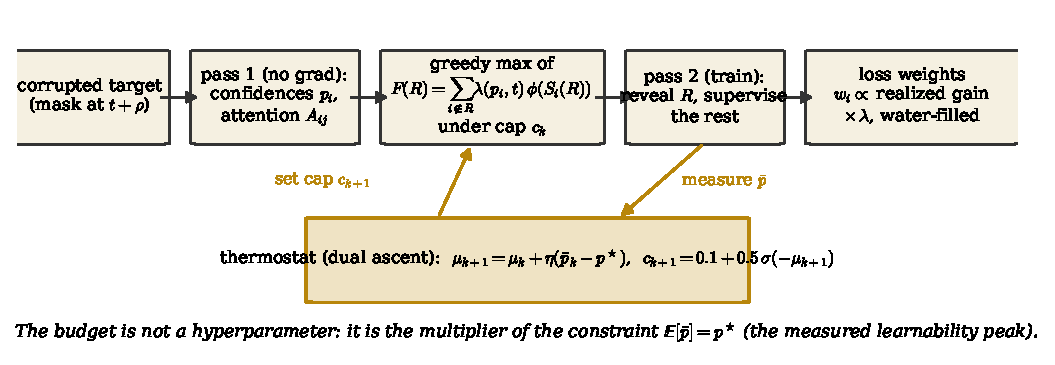
\includegraphics[width=\textwidth]{figs/fig_overview.pdf}
\caption{\textbf{GoldiMask with the dual-cap thermostat.} Each training step runs the two-pass structure (gradient-free statistics, submodular reveal selection, supervised pass with realized-gain weights); the budget that the selection operates under is not a hyperparameter but the Lagrange multiplier of the constraint $\mathbb{E}[\bar p] = p^\star$, updated by two lines of dual ascent from a quantity the training pass already computes. $p^\star$ is the measured learnability peak---the one number the mechanism needs, and it is read off a 25-GPU-minute diagnostic rather than tuned.}
\label{fig:overview}
\end{figure}

\begin{figure}[t]
\centering
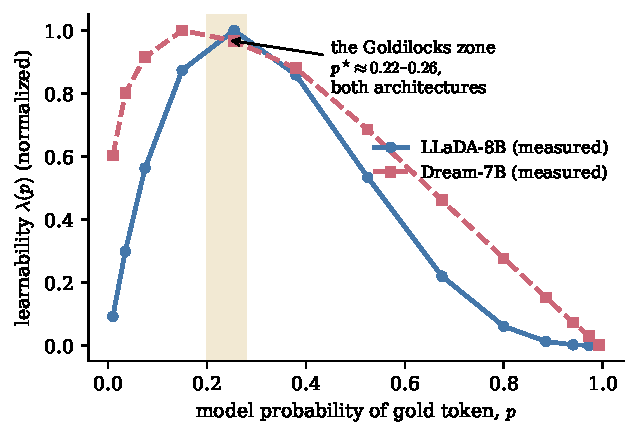
\includegraphics[width=0.6\textwidth]{figs/fig_invariance.pdf}
\caption{\textbf{The learnability peak is architecture-invariant.} The measured curve $\lambda(p)$ (mid-noise bin, each normalized to its maximum) on LLaDA-8B and on Dream-7B---different architectures, different pretraining (Dream is autoregressively initialized)---peaks in the same zone, $p^\star \approx 0.22$--$0.26$. This invariance is the empirical license for the dual-cap constraint: the target the thermostat enforces is a property of masked-diffusion learning, not a per-model tuning.}
\label{fig:invariance}
\end{figure}


\begin{figure}[t]
\centering
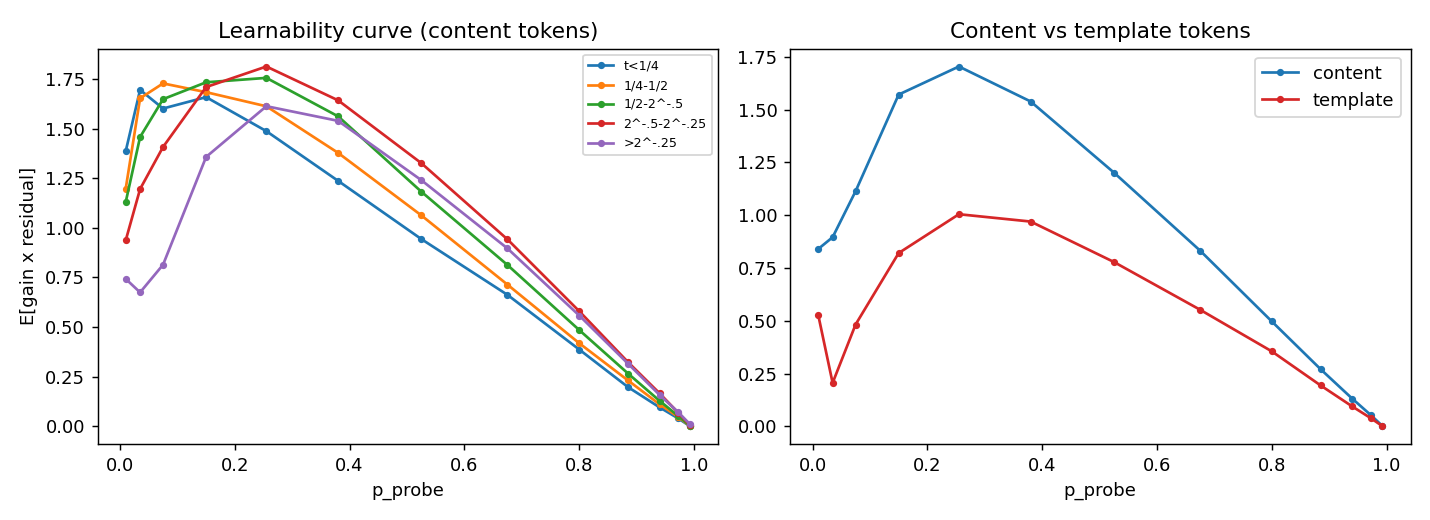
\includegraphics[width=0.86\textwidth]{fig_learnability.png}\\[4pt]
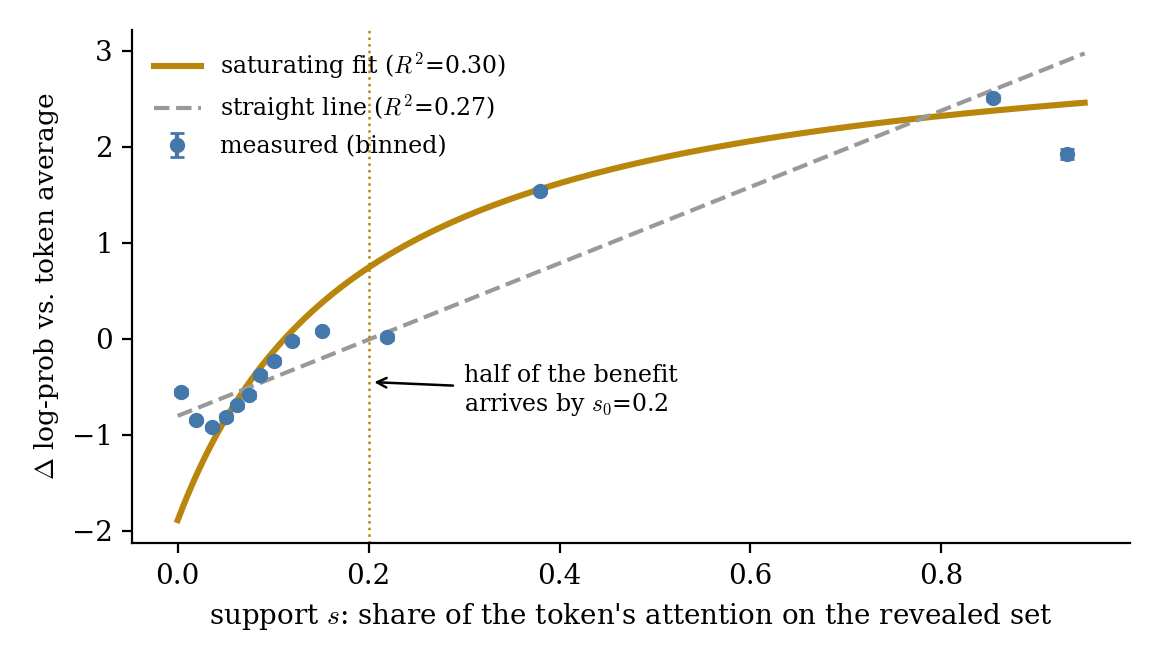
\includegraphics[width=\textwidth]{fig_phi.png}
\caption{\textbf{The two measured curves.} \emph{Top:} the learnability curve $\lambda(p,t)$ over 957{,}563 tokens --- a lopsided inverted U whose peak sits at $p \approx 0.22$ in every noise bin (left), with template tokens carrying little of the mass (right). \emph{Bottom:} the support curve $\phi$ from within-target randomized reveal contrasts (25{,}217 targets $\times$ 8 random sets): monotone in every noise bin, gently saturating, and thirty-fold stronger at high noise --- context identity matters where masking is heavy. Together the two curves fully specify the GoldiMask objective; neither matches any standard hand-designed weighting.}
\label{fig:curves}
\end{figure}

\begin{figure}[t]
\centering
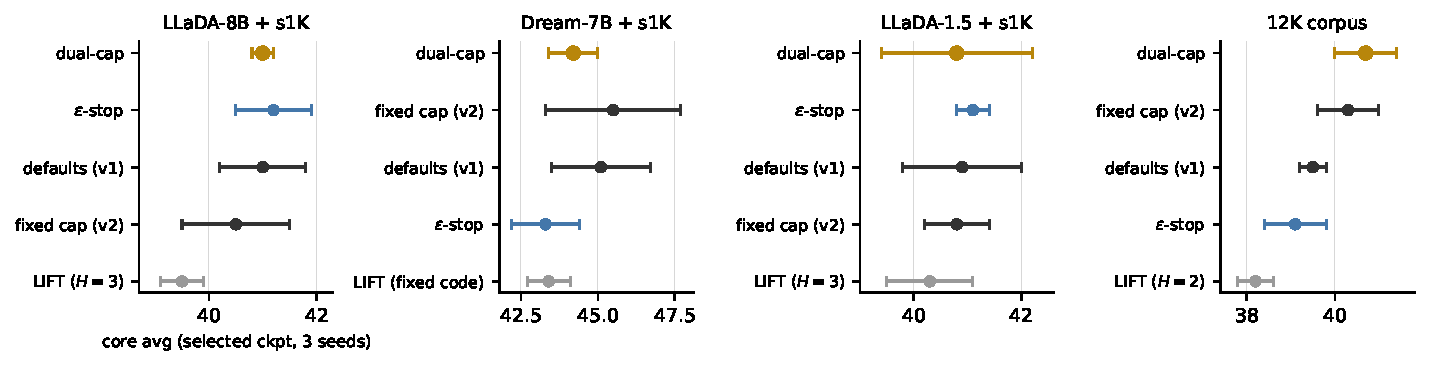
\includegraphics[width=\textwidth]{figs/fig_flagship.pdf}
\caption{\textbf{The flagship across all four settings} (core average, selected checkpoint, mean $\pm$ sd over seeds 42--44). Dual-cap (gold) is the only configuration in the top band everywhere; each setting's local specialist differs ($\varepsilon$-stop on LLaDA-8B, the fixed cap on Dream), and same-harness LIFT (gray) trails on all four. Note the variance: $\pm 0.2$ on LLaDA-8B is the smallest of any configuration we trained.}
\label{fig:flagship}
\end{figure}

\begin{figure}[t]
\centering
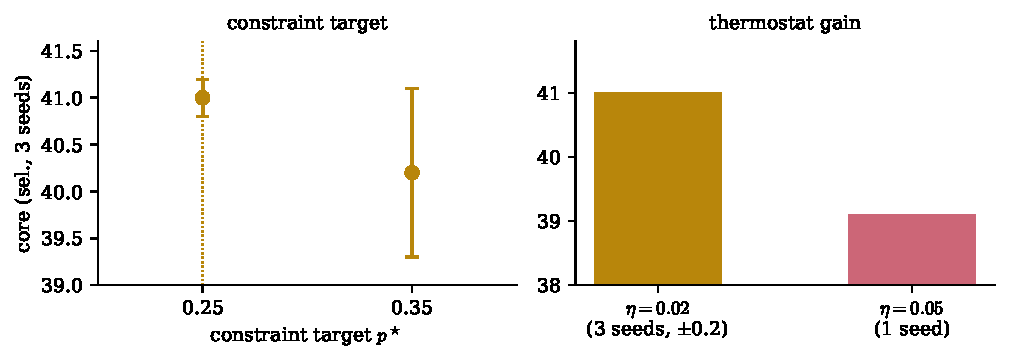
\includegraphics[width=0.78\textwidth]{figs/fig_dose.pdf}
\caption{\textbf{Two causal probes of the thermostat.} \emph{Left:} the dose--response in the constraint target: holding supervised difficulty at the measured peak ($p^\star{=}0.25$) beats holding it above ($0.35$) in both mean and seed variance---the constraint's location does causal work. \emph{Right:} the dual-ascent gain is an operating condition: $\eta = 0.05$ overshoots the equilibrium the proposition describes ($39.1$ at seed 42, versus $41.0 \pm 0.2$ at the default $\eta = 0.02$).}
\label{fig:dose}
\end{figure}

\begin{figure}[t]
\centering
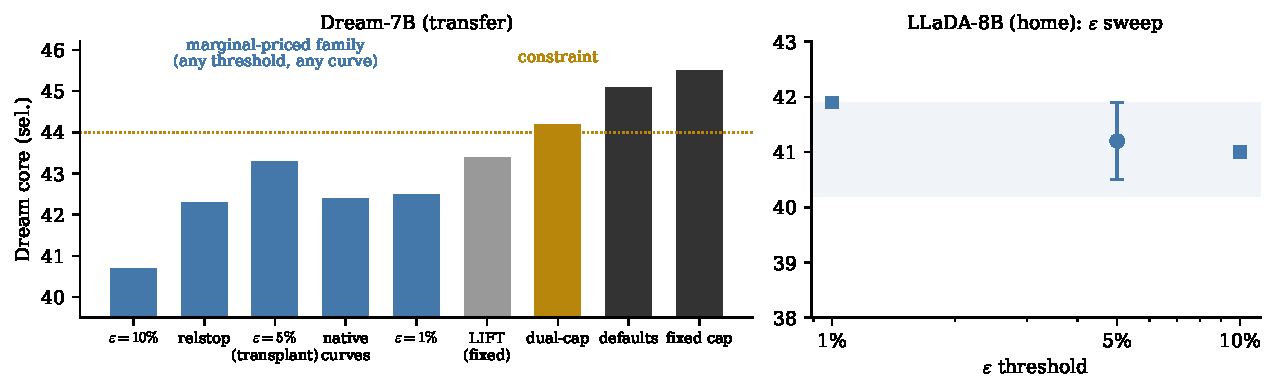
\includegraphics[width=\textwidth]{figs/fig_dichotomy.pdf}
\caption{\textbf{The transfer dichotomy.} \emph{Left:} on Dream-7B, every member of the marginal-priced family (blue: thresholds $1\%/5\%/10\%$, a scale-free variant, and retraining with natively re-measured Dream curves) plateaus $1$--$4$ points below the fixed-budget configurations, while the constraint-based dual-cap (gold) transfers into the top band unchanged. \emph{Right:} on its home model the same $\varepsilon$ family is flat across a tenfold threshold range---the failure is the family's, not the constant's.}
\label{fig:dichotomy}
\end{figure}

\begin{figure}[t]
\centering
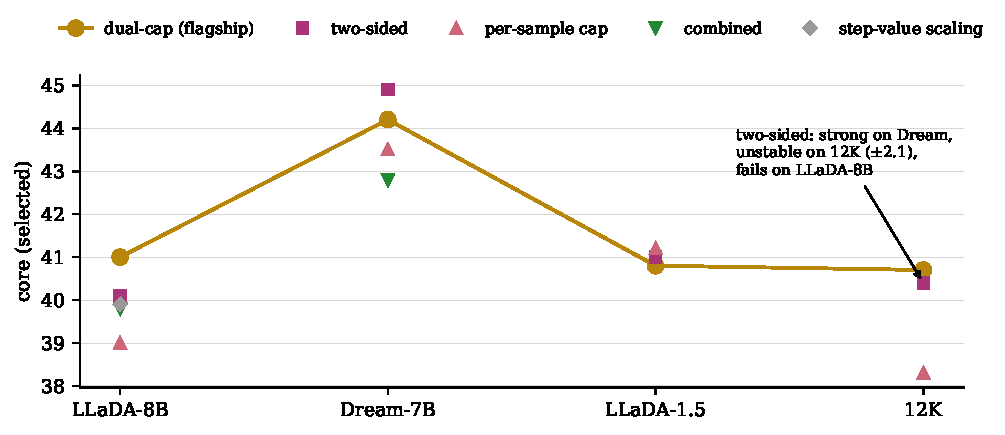
\includegraphics[width=0.9\textwidth]{figs/fig_refute.pdf}
\caption{\textbf{The refutation campaign at a glance} (core, selected checkpoint). Four independently-motivated refinements versus the flagship (gold line) across the four settings. None beats the flagship on its own terms; the one local exception (two-sided on Dream) comes with instability elsewhere and is reported as a finding about architecture-dependence.}
\label{fig:refute}
\end{figure}

\section{Hardware-layout equivalence: 1 GPU versus 4 GPUs}
\label{app:layout}

The refutation campaign of Section~\ref{sec:refute} was trained on single GPUs (batch 1, gradient accumulation 8), while the earlier campaigns used 4-GPU data parallelism (batch 1 per rank, accumulation 2)---the same global batch of 8 and identical hyperparameters, but not the same execution: floating-point reduction order, sampler sharding, and per-example corruption-noise streams all differ, so same-seed runs are not bitwise-identical across layouts. Cross-layout comparisons are only honest if the layouts are \emph{statistically} equivalent, and we measured this directly rather than assuming it: one $\varepsilon$-stop configuration and the full dual-cap slates on LLaDA-1.5 and 12K were trained on \emph{both} layouts at identical seeds.

Result (Figure~\ref{fig:aa}): across all fourteen completed pairs the gaps are $+0.6, +0.2, +1.6, +0.2, -0.4, -1.9, -0.3, -0.8, +0.1, +0.5, +1.6, -0.6, +2.4, +0.9$ core points (positive = 4-GPU higher): both signs (8/6), mean $+0.29$ with sd $1.13$ ($t \approx 1.0$, not significant), every gap inside the configuration's own cross-seed spread, and the LLaDA-1.5 selected means coincide exactly ($40.8$ versus $40.8$). Two mild sub-patterns appear and point in \emph{opposite} directions---the 12K selected column favors 4-GPU ($+1.4$ mean; higher checkpoint peaks on the long schedule) while the LLaDA-1.5 final column favors 1-GPU ($41.4 \pm 0.3$ versus $40.9 \pm 0.5$)---which is the signature of noise, not of a systematic layout effect. We conclude the two layouts draw from the same result distribution, differing like a seed re-draw; no comparison in this paper is confounded by hardware layout.

\begin{figure}[h]
\centering
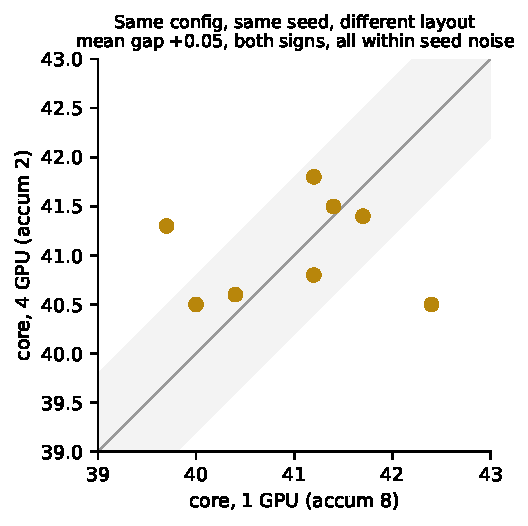
\includegraphics[width=0.5\textwidth]{figs/fig_aa.pdf}
\caption{\textbf{Layout equivalence.} Paired same-configuration, same-seed runs trained on 1 GPU (accumulation 8) versus 4 GPUs (accumulation 2). All fourteen pairs scatter around the identity line within the shaded typical seed-noise band ($\pm 0.8$); the mean paired gap is $+0.29$ core points (not significant).}
\label{fig:aa}
\end{figure}

\section{The checkpoint selector, and the temperature sweep}
\label{app:selector}
The original pipeline selects checkpoints by validation loss on 10 examples with freshly drawn corruption noise; the draw includes near-zero noise levels whose $1/t$ scaling produces loss spikes of two orders of magnitude, and curve-weighted GoldiMask runs exhibit visibly smoother validation trajectories. Two consequences appear throughout the paper. First, per-benchmark scores swing $\pm 3$ points with checkpoint choice for every method (e.g., our LLaDA-1.5 run reads 40.6 / 40.4 / 39.5 / 41.4 core at checkpoints 700 / 1200 / 1900 / 2480). Second, the selector helps some methods and not others: it adds nothing over the final checkpoint for LIFT ($H{=}3$) while consistently locating GoldiMask defaults' stronger checkpoints (Section~\ref{sec:experiments}).

The AIME sampling-temperature sweep of Section~\ref{sec:aime} (seed 42, pass@16 over 16 runs, AIME'24/'25):

\begin{center}
\begin{tabular}{lccc}
\toprule
 & $T{=}0.1$--$0.2$ (protocol) & $T{=}0.3$ & $T{=}0.5$ \\
\midrule
GoldiMask (defaults, sel.)   & 6.7 / 0.0 & 10.0 / 3.3 & 13.3 / 3.3 \\
GoldiMask (full fading, final) & 6.7 / 3.3 & 10.0 / 0.0 & --- \\
LIFT ($H{=}3$, sel.)         & 13.3 / 3.3 & 13.3 / --- & 16.7 / 0.0 \\
\bottomrule
\end{tabular}
\end{center}

The recovery is monotone in temperature for both methods, larger for the sharper model ($+6.6$ versus $+3.4$ on AIME'24), and the summed AIME'24$+$'25 tails at $T{=}0.5$ are 16.6 (ours) versus 16.7 (LIFT).

\end{document}
